\documentclass[12pt,a4paper]{article}

\usepackage[utf8]{inputenc}
\usepackage[T1]{fontenc}
\usepackage{lmodern}
\usepackage{textcomp}
\usepackage{graphicx}
\usepackage{amsfonts}
\usepackage{amssymb}
\usepackage{amsmath}
\usepackage{float}
\usepackage{needspace}
\graphicspath{ {figures/} }
\usepackage{geometry}
\usepackage{booktabs}
\usepackage{longtable}
\usepackage{array}
\usepackage[english]{babel}
\usepackage{listings}
\usepackage{color}
\usepackage[hidelinks]{hyperref}
\definecolor{dkgreen}{rgb}{0,0.6,0}
\definecolor{gray}{rgb}{0.5,0.5,0.5}
\definecolor{mauve}{rgb}{0.58,0,0.82}
\lstset{frame=tb,
  aboveskip=3mm,
  belowskip=3mm,
  showstringspaces=false,
  columns=fixed,
  basewidth=0.52em,
  basicstyle={\footnotesize\ttfamily},
  numbers=none,
  numberstyle=\tiny\color{gray},
  keywordstyle=\color{blue},
  commentstyle=\color{dkgreen},
  stringstyle=\color{mauve},
  breaklines=true,
  breakatwhitespace=true,
  tabsize=3,
  upquote=true,
  keepspaces=true,
  escapeinside={(*@}{@*)}
}
\setlength{\parindent}{0pt}
\setlength{\parskip}{0.6em}
\setlength{\LTpre}{0.4em}
\setlength{\LTpost}{0.4em}
\renewcommand{\arraystretch}{1.25}
\setcounter{tocdepth}{2}
\hypersetup{pdftitle={CALPHAD Study Guide: From Gibbs Energy to the KKS Server}, pdfauthor={Gaurav Rathod}}
\sloppy

\title{\textbf{CALPHAD Study Guide} \\ \vspace{0.3cm} \textit{From Gibbs Energy to the KKS Server} \\}
\author{}
\date{}

\begin{document}

\maketitle
\vspace{-1.5cm}
\begin{center}
    \large{\textbf{Prepared for} \\ Gaurav Rathod \\}
    \vspace{1cm}
    \large{\textbf{Companion reference} \\ \href{https://claude.ai/artifact/DYaPx84Vvd9nVVGhyTVKLF}{\textit{CALPHAD Server \& KKS Framework Guide}} \\}
    \vspace{1cm}
    \textit{6 November 2026} \\
\end{center}

\pagebreak
\tableofcontents

\newpage
\newgeometry{top = 25mm, bottom = 20mm, right = 25mm, left = 25mm}

This guide takes you from reading a phase diagram to understanding every call in the CALPHAD server and its KKS module, one idea at a time. Each part builds on the one before, runs real code on the bundled Cu--Ni and Ni--Al databases, and ends with exercises; the answers are at the end.


\needspace{10\baselineskip}
\section*{Roadmap}
\addcontentsline{toc}{section}{Roadmap}
Nine parts take you from the physics to the code. Parts 1--4 are the science, 5--7 are pycalphad and the framework, 8 is phase-field and KKS, and 9 ties it together. Each part assumes only the parts before it. The companion reference is \href{https://claude.ai/artifact/DYaPx84Vvd9nVVGhyTVKLF}{\textit{CALPHAD Server \& KKS Framework Guide}}; the right-hand column says which of its sections each part prepares you for.

Throughout this guide, ``Reference \S5'' means Section~5 of that reference guide; \S{} is simply the section sign.

\begingroup\small
\begin{longtable}{>{\raggedright\arraybackslash}p{0.161\linewidth}>{\raggedright\arraybackslash}p{0.247\linewidth}>{\raggedright\arraybackslash}p{0.297\linewidth}>{\raggedright\arraybackslash}p{0.188\linewidth}}
\toprule
\textbf{Part} & \textbf{You learn} & \textbf{Afterwards you can} & \textbf{Prepares you for} \\
\midrule
\endhead
1. Gibbs energy & G = H \(-\) TS; the lowest G wins; G against composition & Explain why a liquid freezes on cooling & The vocabulary of everything else \\
2. From G curves to the phase diagram & Chemical potential, common tangent, tie lines, lever rule & Check an API 1 result by hand & Reference \S{}5 (API 1) and \S{}6 (API 2) \\
3. The CALPHAD idea & How a database writes G for each phase; sublattices; ordering & Read ``site fraction'', ``ordered'', ``disordered'' in results & Reference \S{}3 (conventions) \\
4. Reading a TDB file & The file format, line by line & Open any TDB and find its phases and parameters & Reference \S{}4 (databases) \\
5. pycalphad hands-on & \texttt{Database}, \texttt{equilibrium}, \texttt{calculate}, \texttt{Model} & Compute an equilibrium yourself, no server & \texttt{calphad\_\allowbreak{}core.\allowbreak{}py} \\
6. Where pycalphad needs help & Sampling, local minima, phase names & Interpret \texttt{stability\_\allowbreak{}check}, \texttt{state}, \texttt{equivalent\_\allowbreak{}to} & Reference \S{}5 (stability check), \S{}12 \\
7. The framework layer by layer & How each API is built; HTTP and JSON & Read \texttt{calphad\_\allowbreak{}core.\allowbreak{}py} and \texttt{calphad\_\allowbreak{}server.\allowbreak{}py}; call the APIs from any language & Reference \S{}4--7 and \S{}10 \\
8. Phase-field and KKS & Order parameter, diffuse interface, the KKS split & Read \texttt{calphad\_\allowbreak{}kks.\allowbreak{}py} and the 1-D demo & Reference \S{}8, \S{}9, \S{}11 \\
9. Putting it together & End-to-end tasks & Plan the thermodynamic inputs of your Ni--Al dendrite model & The whole reference \\
\bottomrule
\end{longtable}
\endgroup

\needspace{7\baselineskip}
\subsection*{How to work through it}
\addcontentsline{toc}{subsection}{How to work through it}
\begin{enumerate}
\item Read one part.
\item Run its code. Every snippet was run while writing this guide, and its real output is shown under it.
\item Do its exercises before looking at the answers at the end.
\end{enumerate}

\needspace{7\baselineskip}
\subsection*{Before you start}
\addcontentsline{toc}{subsection}{Before you start}
Unzip \texttt{calphad\_\allowbreak{}server.\allowbreak{}zip}, open a terminal in the \texttt{calphad\_\allowbreak{}server} folder and install the two packages the lessons use:

\begin{lstlisting}[basicstyle={\footnotesize\ttfamily},language=bash]
pip install pycalphad matplotlib
python -c "import pycalphad; print(pycalphad.__version__)"
# 0.11.2
\end{lstlisting}
Run every snippet from inside that folder, in a Python file or a Jupyter notebook, so the database files are found. Snippets in one part build on each other, so run them in order in the same session.


\needspace{10\baselineskip}
\section*{Part 1 --- Gibbs energy: why one phase wins}
\addcontentsline{toc}{section}{Part 1 --- Gibbs energy: why one phase wins}
At a given temperature and pressure, a material settles into whichever state has the lowest Gibbs energy, G. Every number the server returns is either a value of G or something worked out from it.


\needspace{7\baselineskip}
\subsection*{G = H \texorpdfstring{\(-\)}{-} TS}
\addcontentsline{toc}{subsection}{G = H \texorpdfstring{\(-\)}{-} TS}
\begin{itemize}
\item \textbf{H, the enthalpy}, is roughly the energy held in the bonds. In a crystal the atoms sit in a tight, ordered arrangement, so a solid has lower H than its liquid.
\item \textbf{S, the entropy}, measures disorder: how many ways the atoms can be arranged. A liquid is more disordered, so it has higher S.
\item \textbf{\(-\)TS grows with temperature.} At low T the H term wins and the solid has the lower G. At high T the \(-\)TS term wins and the liquid does. The melting point is the temperature where the two are equal.
\end{itemize}
Here is that crossing for pure copper, computed from the Cu--Ni database you have:

\begin{figure}[htbp]
\centering
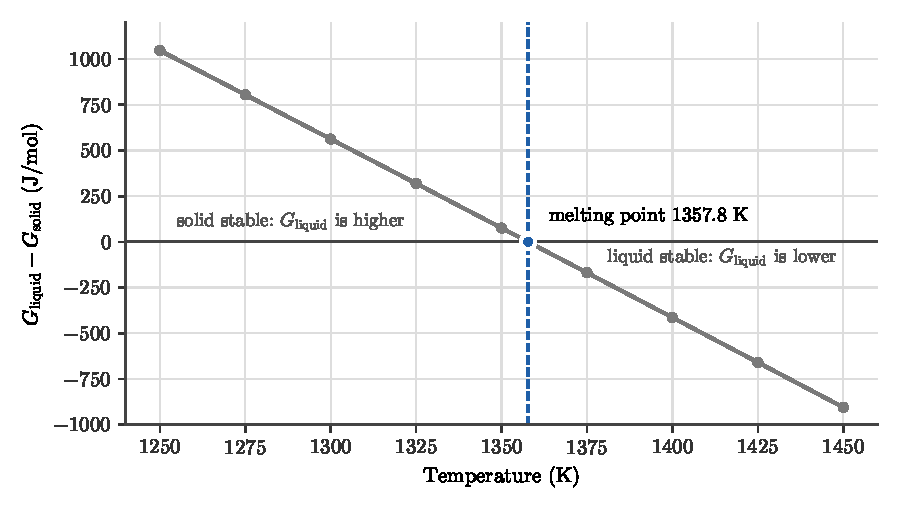
\includegraphics[width=0.85\textwidth]{cu_melting.pdf}
\caption{Copper melts where the liquid's G drops below the solid's. Pure Cu from \texttt{cuni\_cost507.tdb} (COST 507), computed with pycalphad, 1250--1450~K.}
\label{fig:cu-melting}
\end{figure}
\begingroup\small
\begin{longtable}{>{\raggedright\arraybackslash}p{0.120\linewidth}>{\raggedright\arraybackslash}p{0.295\linewidth}>{\raggedright\arraybackslash}p{0.245\linewidth}>{\raggedright\arraybackslash}p{0.234\linewidth}}
\toprule
\textbf{T (K)} & \textbf{G of solid (FCC), J/mol} & \textbf{G of liquid, J/mol} & \textbf{Lower} \\
\midrule
\endhead
1300 & \(-\)67 060.8 & \(-\)66 498.2 & solid, by 562.6 \\
1358 & \(-\)71 321.1 & \(-\)71 323.3 & about equal \\
1400 & \(-\)74 452.4 & \(-\)74 865.9 & liquid, by 413.4 \\
\bottomrule
\end{longtable}
\endgroup
The crossing, 1357.8 K, is copper's measured melting point: the database was fitted to reproduce it.

\textbf{Units and the reference.} G is in joules per mole of atoms. A value such as \(-\)67 060.8 J/mol is measured from a reference state, like a height measured from sea level, so it means nothing on its own. Differences between phases, compositions or temperatures are what matter.


\needspace{7\baselineskip}
\subsection*{In an alloy, G depends on composition}
\addcontentsline{toc}{subsection}{In an alloy, G depends on composition}
Add a second element and each phase gets its own G that changes with the composition x (the mole fraction of the second element): a curve, not a single number. The simplest model is the \textbf{ideal solution}:

\begin{equation*}
G(x) = (1 - x)\,G_A + x\,G_B + RT\left[x \ln x + (1 - x)\ln(1 - x)\right]
\end{equation*}
\begin{itemize}
\item The first two terms are a straight line between the pure-element values \(G_{A}\) and \(G_{B}\).
\item The last term is the \textbf{entropy of mixing}. Mixing two kinds of atom adds disorder, so this term is always negative. It is deepest at x = 0.5.
\item Its slope becomes infinitely steep as x approaches 0 or 1. The first few solute atoms always lower G, which is why no real metal is perfectly pure.
\end{itemize}
Real alloys add an \textbf{excess} term for how much A and B atoms like or dislike each other. That term is what CALPHAD fits to experiments (Part 3).

\begin{lstlisting}[basicstyle={\footnotesize\ttfamily},language=Python]
import numpy as np

R = 8.314462618          # gas constant, J/(mol K)

def g_mix_ideal(x, T):
    """Ideal Gibbs energy of mixing, J/mol: R T [x ln x + (1-x) ln(1-x)]"""
    return R * T * (x * np.log(x) + (1 - x) * np.log(1 - x))

for x in (0.1, 0.5):
    print(f"ideal mixing at x = {x}, 1500 K: {g_mix_ideal(x, 1500):.1f} J/mol")
# ideal mixing at x = 0.1, 1500 K: -4054.3 J/mol
# ideal mixing at x = 0.5, 1500 K: -8644.7 J/mol
\end{lstlisting}
The copper numbers above came from this short pycalphad script. Each piece of its syntax is explained in Part 5; for now, read it as ``evaluate the G of pure Cu in each phase at temperature T'':

\begin{lstlisting}[basicstyle={\scriptsize\ttfamily},language=Python]
from pycalphad import Database, calculate

db = Database("cuni_cost507.tdb")
for T in (1300, 1358, 1400):
    g_fcc = calculate(db, ["CU", "NI", "VA"], "FCC_A1", T=T, P=101325, N=1,
                      points=np.array([[1 - 1e-12, 1e-12, 1.0]]), output="GM").GM.values.item()
    g_liq = calculate(db, ["CU", "NI", "VA"], "LIQUID", T=T, P=101325, N=1,
                      points=np.array([[1 - 1e-12, 1e-12]]), output="GM").GM.values.item()
    print(f"T = {T} K: G_fcc = {g_fcc:10.1f}  G_liquid = {g_liq:10.1f}  difference = {g_liq - g_fcc:7.1f} J/mol")
# T = 1300 K: G_fcc =   -67060.8  G_liquid =   -66498.2  difference =   562.6 J/mol
# T = 1358 K: G_fcc =   -71321.1  G_liquid =   -71323.3  difference =    -2.2 J/mol
# T = 1400 K: G_fcc =   -74452.4  G_liquid =   -74865.9  difference =  -413.4 J/mol
\end{lstlisting}

\needspace{7\baselineskip}
\subsection*{Key ideas}
\begin{itemize}
\item At fixed T and P, the lowest G wins.
\item G = H \(-\) TS. Raising T shifts the balance from H, which favours solids, to S, which favours liquids.
\item In an alloy, G is a curve over composition, one curve per phase.
\item Energies are J per mole of atoms from a reference. Compare them; never read them alone.
\end{itemize}

\needspace{7\baselineskip}
\subsection*{Exercises}
\begin{itemize}
\item \textbf{1.1} From the table, by how much is solid copper more stable than liquid at 1300 K? Which phase is stable at 1400 K, and by how much?
\item \textbf{1.2} Use \texttt{g\_\allowbreak{}mix\_\allowbreak{}ideal} to compute the ideal mixing term at x = 0.25 and 1500 K. Is it more or less negative than at x = 0.1?
\item \textbf{1.3} In the ideal model, why does adding a tiny amount of solute to a pure metal always lower G? Hint: look at the slope of x ln x near x = 0.
\item \textbf{1.4} In Figure~\ref{fig:cu-melting}, what does a positive value of G liquid \(-\) G solid mean physically?
\end{itemize}

\needspace{10\baselineskip}
\section*{Part 2 --- From G curves to the phase diagram}
\addcontentsline{toc}{section}{Part 2 --- From G curves to the phase diagram}
Where two phases' G curves overlap, an alloy can lower its G by splitting into two phases whose compositions are where one straight line touches both curves: the \textbf{common tangent}. That single construction draws every two-phase region of a phase diagram, and API 1 is a machine for finding it.


\needspace{7\baselineskip}
\subsection*{Why splitting can lower G}
\addcontentsline{toc}{subsection}{Why splitting can lower G}
\begin{itemize}
\item A mixture of two phases has a total G on the straight line joining the two phases' points (x, G): it is a weighted average.
\item If that line passes below every single-phase curve at the alloy's composition, the mixture wins.
\item The lowest such line touches both curves. The touch points are the two phase compositions, and they are the same for every alloy between them at that temperature. Only the amounts of each phase change.
\end{itemize}

\needspace{7\baselineskip}
\subsection*{See it at 1500 K}
\addcontentsline{toc}{subsection}{See it at 1500 K}
\begin{figure}[htbp]
\centering
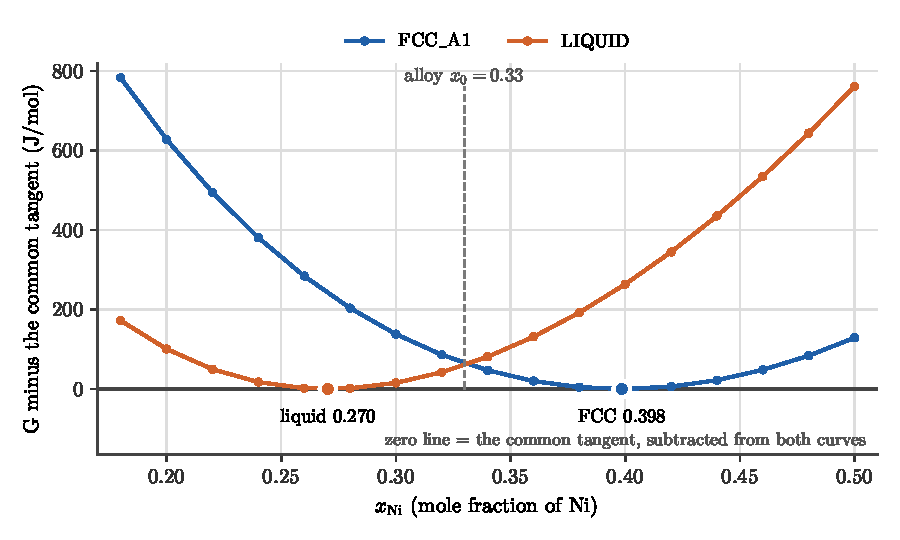
\includegraphics[width=0.85\textwidth]{cuni_g_1500.pdf}
\caption{At 1500~K one straight line touches both Gibbs energy curves. \texttt{cuni\_cost507.tdb} at 1500~K: API~3 (\texttt{energy\_surface}) minus the API~1 tangent, \(x_{\mathrm{Ni}}\) = 0.18--0.50.}
\label{fig:cuni-g}
\end{figure}
The raw curves are almost straight lines tens of kJ/mol below zero, so the touching is invisible. Figure~\ref{fig:cuni-g} subtracts the tangent line from both curves. Subtracting the same straight line from every curve changes no comparison, so the tangent becomes the zero line and both curves rest on it.

At the alloy composition 0.33, the liquid curve is about 60 J/mol above zero and the FCC curve about 65 J/mol above it. Those are exactly the \texttt{GM\_\allowbreak{}above\_\allowbreak{}equilibrium} values API 2 reports in Example 6.1 of the reference: the cost of forcing the whole alloy into one phase.


\needspace{7\baselineskip}
\subsection*{Chemical potential}
\addcontentsline{toc}{subsection}{Chemical potential}
The tangent line is written with two numbers, its heights at the pure-element ends:

\begin{equation*}
G_{\text{line}}(x) = (1 - x)\,\mu_{Cu} + x\,\mu_{Ni}
\end{equation*}
\begin{itemize}
\item \(\mu_{\mathrm{Cu}}\) and \(\mu_{\mathrm{Ni}}\) are the \textbf{chemical potentials}, in J/mol. \(\mu_{\mathrm{Ni}}\) is the change in G when one mole of Ni is added to a large amount of the material.
\item Atoms move from where their \(\mu\) is higher to where it is lower. At equilibrium each element has the same \(\mu\) in every phase, so the common tangent and ``equal \(\mu\) everywhere'' are the same statement.
\item At 1500 K, API 1 returns \(\mu_{\mathrm{Cu}}\) = \(-\)86 428.34 and \(\mu_{\mathrm{Ni}}\) = \(-\)88 267.79 J/mol in \texttt{chemical\_\allowbreak{}potentials}.
\item The tangent's slope, \(\mu_{\mathrm{Ni}}\) \(-\) \(\mu_{\mathrm{Cu}}\) = \(-\)1839.45 J/mol, is the \textbf{diffusion potential}. Part 8 uses it: the KKS model makes it equal in both phases at every point of the interface.
\end{itemize}

\needspace{7\baselineskip}
\subsection*{From one temperature to the whole diagram}
\addcontentsline{toc}{subsection}{From one temperature to the whole diagram}
Repeat the construction at each temperature. The liquid touch points trace the \textbf{liquidus}, and the solid touch points trace the \textbf{solidus}:

\begin{figure}[htbp]
\centering
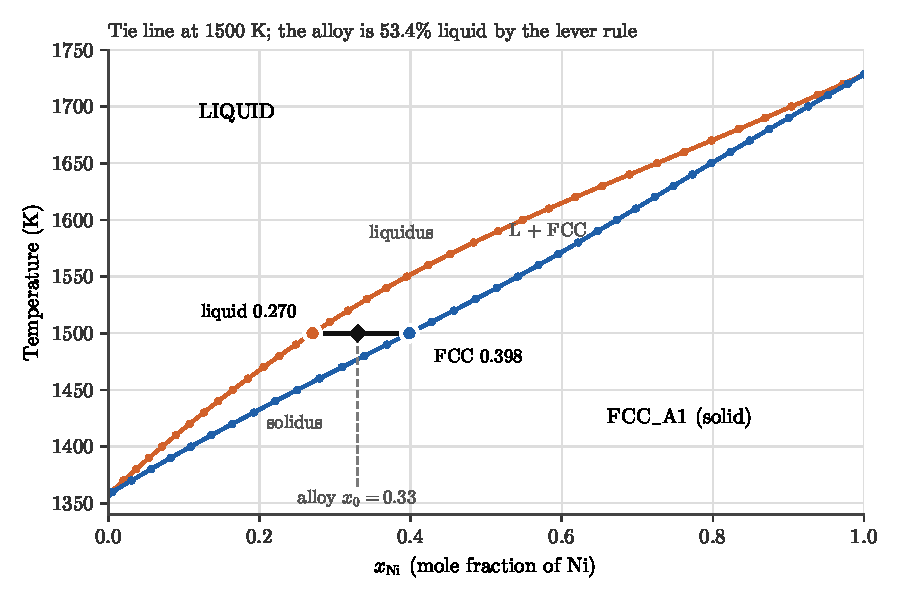
\includegraphics[width=0.85\textwidth]{cuni_phase_diagram.pdf}
\caption{Reading the Cu--Ni phase diagram at 1500~K. Tie lines every 10~K from pycalphad equilibrium on \texttt{cuni\_cost507.tdb}; melting points of Cu and Ni from pycalphad.}
\label{fig:cuni-pd}
\end{figure}
The horizontal line at 1500 K is the \textbf{tie line}. Its ends are the two touch points in Figure~\ref{fig:cuni-g}. The curves meet the axes at copper's melting point, 1357.8 K, and nickel's, 1728.3 K.


\needspace{7\baselineskip}
\subsection*{The lever rule}
\addcontentsline{toc}{subsection}{The lever rule}
Mass balance sets how much of each phase there is. With \(f_{L}\) the liquid fraction, \(f_{L}\) \(x_{L}\) + (1 \(-\) \(f_{L}\)) \(x_{S}\) = x\(_{0}\), so:

\begin{equation*}
f_L = \frac{x_S - x_0}{x_S - x_L} = \frac{0.3985 - 0.33}{0.3985 - 0.2703} = 0.534
\end{equation*}
53.4\% of the atoms are in the liquid: exactly the \texttt{fraction} API 1 returns for \texttt{LIQUID}.


\needspace{7\baselineskip}
\subsection*{Check API 1 by hand}
\addcontentsline{toc}{subsection}{Check API 1 by hand}
Save this as a file inside the \texttt{calphad\_\allowbreak{}server} folder (or run it in a notebook started there):

\begin{lstlisting}[basicstyle={\scriptsize\ttfamily},language=Python]
from calphad_core import CalphadSystem

s = CalphadSystem.from_file("cuni_cost507.tdb")
r = s.equilibrium({"NI": 0.33}, T=1500, balance="CU")["results"]

mu = r["chemical_potentials"]
print("chemical potentials:", {k: round(v, 2) for k, v in mu.items()})
for p in r["phases"]:
    print(p["phase"], "fraction", round(p["fraction"], 4), "x_Ni", round(p["composition"]["NI"], 4))
print("slope of the tangent (mu_Ni - mu_Cu):", round(mu["NI"] - mu["CU"], 2), "J/mol")

x0 = 0.33
xL = next(p["composition"]["NI"] for p in r["phases"] if p["phase"] == "LIQUID")
xS = next(p["composition"]["NI"] for p in r["phases"] if p["phase"] == "FCC_A1")
print(f"lever rule: liquid fraction = {(xS - x0) / (xS - xL):.4f}")
\end{lstlisting}
\begin{lstlisting}[basicstyle={\footnotesize\ttfamily}]
chemical potentials: {'CU': -86428.34, 'NI': -88267.79}
LIQUID fraction 0.5344 x_Ni 0.2703
FCC_A1 fraction 0.4656 x_Ni 0.3985
slope of the tangent (mu_Ni - mu_Cu): -1839.45 J/mol
lever rule: liquid fraction = 0.5344
\end{lstlisting}
The \texttt{next(.\allowbreak{}.\allowbreak{}.\allowbreak{} for p in .\allowbreak{}.\allowbreak{}.\allowbreak{} if .\allowbreak{}.\allowbreak{}.\allowbreak{})} lines pick the one phase entry with a given name out of the \texttt{phases} list.


\needspace{7\baselineskip}
\subsection*{Key ideas}
\begin{itemize}
\item Two phases coexist where one straight line, the common tangent, touches both G curves. The touch points are their compositions.
\item The tangent's ends are the chemical potentials; its slope is the diffusion potential.
\item Equilibrium means each element has the same \(\mu\) in every phase.
\item Tie-line ends at each T trace the liquidus and solidus; the lever rule gives the amounts.
\end{itemize}

\needspace{7\baselineskip}
\subsection*{Exercises}
\begin{itemize}
\item \textbf{2.1} Read the liquid and FCC compositions at 1550 K off the phase diagram (Figure~\ref{fig:cuni-pd}). Use the lever rule to find the liquid fraction of Cu--50Ni at 1550 K, then check with \texttt{s.\allowbreak{}equilibrium(\{\textquotedbl{}NI\textquotedbl{}: 0.\allowbreak{}5\},\allowbreak{} T=1550,\allowbreak{} balance=\textquotedbl{}CU\textquotedbl{})}.
\item \textbf{2.2} At 1500 K, is Cu--20Ni one phase or two? Which one? Answer from Figure~\ref{fig:cuni-pd} first, then check with API 1.
\item \textbf{2.3} Suppose \(\mu_{\mathrm{Ni}}\) were lower in the FCC than in the liquid. Which way would Ni atoms move, and when would they stop?
\item \textbf{2.4} From Figure~\ref{fig:cuni-g}, about how much does G drop when Cu--33Ni splits into liquid + FCC instead of staying all liquid?
\end{itemize}

\needspace{10\baselineskip}
\section*{Part 3 --- The CALPHAD idea}
\addcontentsline{toc}{section}{Part 3 --- The CALPHAD idea}
CALPHAD (CALculation of PHAse Diagrams) writes the Gibbs energy of every phase as a formula with a handful of parameters fitted to experiments and first-principles calculations. Once G is known for every phase, Part 2's machinery gives phase diagrams, metastable states and driving forces at any composition and temperature, including ones nobody measured.


\needspace{7\baselineskip}
\subsection*{The workflow}
\addcontentsline{toc}{subsection}{The workflow}
\begin{enumerate}
\item \textbf{Collect data} for the pure elements and for each binary and ternary system: melting points, phase boundaries, heats of mixing, energies from first-principles (DFT) calculations.
\item \textbf{Assess} each system: choose a model for each phase and fit its parameters to that data.
\item \textbf{Store} all the parameters in a database file, the TDB (Part 4).
\item \textbf{Compute}: software such as pycalphad or Thermo-Calc finds the arrangement of phases with the lowest total G.
\end{enumerate}
The method's strength is extrapolation. A ternary database is mostly its three binary assessments plus a few ternary parameters, and it still predicts ternary phase diagrams well.


\needspace{7\baselineskip}
\subsection*{A solution phase in four terms}
\addcontentsline{toc}{subsection}{A solution phase in four terms}
For a phase where all atoms share one kind of site, such as the liquid or simple FCC:

\begin{equation*}
G = \sum_i x_i\,{}^{\circ}G_i(T) \;+\; RT\sum_i x_i \ln x_i \;+\; {}^{E}G \;+\; G_{\text{mag}}
\end{equation*}
\begingroup\small
\begin{longtable}{>{\raggedright\arraybackslash}p{0.102\linewidth}>{\raggedright\arraybackslash}p{0.604\linewidth}>{\raggedright\arraybackslash}p{0.214\linewidth}}
\toprule
\textbf{Term} & \textbf{What it describes} & \textbf{Key in pycalphad's \texttt{Model.\allowbreak{}models}} \\
\midrule
\endhead
\(^{\circ}\)G\(_{i}\)(T) & Pure element i in this phase's crystal structure, a polynomial in T & \texttt{ref} \\
RT \(\Sigma\) x\(_{i}\) ln x\(_{i}\) & Ideal mixing (Part 1) & \texttt{idmix} \\
\(^{E}\)G & Excess: how much the atoms like or dislike each other & \texttt{xsmix} \\
\(G_{\mathrm{mag}}\) & Magnetic ordering, for ferromagnetic phases such as FCC Ni & \texttt{mag} \\
\bottomrule
\end{longtable}
\endgroup
The excess term is almost always a \textbf{Redlich--Kister} polynomial:

\begin{equation*}
{}^{E}G = x_A\,x_B \sum_{k} L_k\,(x_A - x_B)^k, \qquad L_k = a_k + b_k T
\end{equation*}
\begin{itemize}
\item A positive L\(_{0}\) means A and B atoms dislike each other: the alloy tends to separate, and at low temperature it can form a miscibility gap.
\item A negative L\(_{0}\) means they attract: the alloy tends to order or form compounds.
\item For the Cu--Ni liquid the database gives L\(_{0}\) = 12 048.61 + 1.29893 T and L\(_{1}\) = \(-\)1861.61 + 0.94201 T. At 1500 K that is L\(_{0}\) = 13 997.0 and L\(_{1}\) = \(-\)448.6 J/mol.
\item Worked example at \(x_{\mathrm{Cu}}\) = 0.67, \(x_{\mathrm{Ni}}\) = 0.33 (pycalphad orders the elements alphabetically, so A = Cu): 0.67 \(\times\) 0.33 \(\times\) [13 997.0 + (\(-\)448.6) \(\times\) (0.67 \(-\) 0.33)] = 3061.0 J/mol.
\end{itemize}

\needspace{7\baselineskip}
\subsection*{Real numbers: the four terms for Cu--33Ni at 1500 K}
\addcontentsline{toc}{subsection}{Real numbers: the four terms for Cu--33Ni at 1500 K}
\begingroup\small
\begin{longtable}{>{\raggedright\arraybackslash}p{0.325\linewidth}>{\raggedright\arraybackslash}p{0.298\linewidth}>{\raggedright\arraybackslash}p{0.298\linewidth}}
\toprule
\textbf{Term (J/mol)} & \textbf{LIQUID} & \textbf{FCC\_A1} \\
\midrule
\endhead
\texttt{ref} & \(-\)82 126.9 & \(-\)81 934.4 \\
\texttt{idmix} & \(-\)7909.3 & \(-\)7909.3 \\
\texttt{xsmix} & 3061.0 & 2873.3 \\
\texttt{mag} & 0.0 & 0.0 \\
Total & \(-\)86 975.2 & \(-\)86 970.4 \\
\bottomrule
\end{longtable}
\endgroup
\begin{itemize}
\item Ideal mixing is identical in both phases: it depends only on composition and T.
\item The two totals differ by only 4.8 J/mol. Small differences decide which phase is stable, which is why databases are fitted carefully.
\item The totals are exactly the \texttt{GM} values API 2 reports for this alloy (Example 6.1 of the reference).
\item The magnetic term is zero because FCC Ni is ferromagnetic only below its Curie temperature, 633 K in this database.
\end{itemize}
The code that produced the table (the \texttt{Model} object is explained in Part 5):

\begin{lstlisting}[basicstyle={\footnotesize\ttfamily},language=Python]
from pycalphad import Database, Model, variables as v

db = Database("cuni_cost507.tdb")
x_ni, T = 0.33, 1500.0
for phase in ("LIQUID", "FCC_A1"):
    m = Model(db, ["CU", "NI", "VA"], phase)
    values = {}
    for y in m.site_fractions:                      # e.g. Y(LIQUID,0,CU)
        name = y.species.name
        values[y] = x_ni if name == "NI" else (1 - x_ni if name == "CU" else 1.0)
    values[v.T] = T
    values[v.P] = 101325
    print(phase)
    for key, expr in m.models.items():
        print(f"   {key:6s} {float(expr.xreplace(values)):12.1f} J/mol")
\end{lstlisting}
\begin{lstlisting}[basicstyle={\footnotesize\ttfamily}]
LIQUID
   ref        -82126.9 J/mol
   idmix       -7909.3 J/mol
   xsmix        3061.0 J/mol
   mag             0.0 J/mol
   ...         (2st, ein, vol, ord: 0.0, terms this database does not use)
FCC_A1
   ref        -81934.4 J/mol
   idmix       -7909.3 J/mol
   xsmix        2873.3 J/mol
   mag            -0.0 J/mol
   ...
\end{lstlisting}

\needspace{7\baselineskip}
\subsection*{Phases with sublattices}
\addcontentsline{toc}{subsection}{Phases with sublattices}
Many crystals have more than one kind of site. CALPHAD's \textbf{sublattice model}, also called the compound energy formalism (CEF), gives each kind of site its own occupancy, the \textbf{site fractions} y.

\begin{itemize}
\item \textbf{Notation.} In the Ni--Al database, \texttt{FCC\_\allowbreak{}L12} is (Al,Ni)\(_{0}\).\(_{75}\) (Al,Ni)\(_{0}\).\(_{25}\) (Va)\(_{1}\): three sublattices with 0.75, 0.25 and 1 sites per formula unit. In an L1\(_{2}\) crystal the 0.25 sublattice is the cube corners and the 0.75 sublattice the face centres.
\item \textbf{From site fractions to composition.} Weight each sublattice by its sites and leave out vacancies:
\end{itemize}
\begin{equation*}
x_B = \frac{\sum_s a_s\, y_B^{(s)}}{\sum_s a_s \bigl(1 - y_{Va}^{(s)}\bigr)}
\end{equation*}
\begin{itemize}
\item \textbf{Ordered: \(\gamma '\) (Ni\(_{3}\)Al).} For Ni--25Al at 1600 K, API 2 reports Al 0.0492 on the first sublattice and 0.8524 on the second. \(x_{\mathrm{Al}}\) = 0.75 \(\times\) 0.0492 + 0.25 \(\times\) 0.8524 = 0.25. Al strongly prefers the corner sites: that is ordering.
\item \textbf{Disordered: \(\gamma\).} For Ni--10Al at 1700 K, API 1 reports Al 0.1 on both sublattices. Identical sublattices mean a disordered phase, so this \texttt{FCC\_\allowbreak{}L12} is really \(\gamma\), \texttt{FCC\_\allowbreak{}A1}. That is what the \texttt{state} and \texttt{equivalent\_\allowbreak{}to} fields report.
\item \textbf{Vacancy sublattices.} \texttt{FCC\_\allowbreak{}A1} in the Cu--Ni database is (Cu,Ni)\(_{1}\)(Va)\(_{1}\). The second sublattice is for interstitial atoms such as C or N in steels; here it holds only vacancies, which is why results show \texttt{\{\textquotedbl{}VA\textquotedbl{}: 1.\allowbreak{}0\}} for it.
\item \textbf{Stoichiometric compounds.} \texttt{AL3NI1} is (Al)\(_{0}\).\(_{75}\)(Ni)\(_{0}\).\(_{25}\): one element per sublattice, so exactly one composition. That is why API 2 returns \texttt{null} for it at any other composition.
\end{itemize}

\needspace{7\baselineskip}
\subsection*{Key ideas}
\begin{itemize}
\item A database is a set of fitted G formulas, one per phase.
\item Solution phases: reference + ideal mixing + Redlich--Kister excess (+ magnetic).
\item Sublattice phases track site fractions; different sublattice compositions mean ordering.
\item One database phase can describe both an ordered and a disordered structure.
\end{itemize}

\needspace{7\baselineskip}
\subsection*{Exercises}
\begin{itemize}
\item \textbf{3.1} FCC Cu--Ni has L\(_{0}\) = 8047.72 + 3.42217 T, which is positive. What does that suggest at low temperature? Test it: run \texttt{s.\allowbreak{}equilibrium(\{\textquotedbl{}NI\textquotedbl{}: 0.\allowbreak{}5\},\allowbreak{} T=500,\allowbreak{} balance=\textquotedbl{}CU\textquotedbl{})} on the Cu--Ni database and explain the result.
\item \textbf{3.2} By hand, compute the excess term of the Cu--Ni liquid at \(x_{\mathrm{Ni}}\) = 0.5 and 1500 K. Why does L\(_{1}\) drop out? Check with the \texttt{Model} code.
\item \textbf{3.3} An \texttt{FCC\_\allowbreak{}L12} phase has Al site fractions 0.10 on the first sublattice and 0.70 on the second. What is \(x_{\mathrm{Al}}\)? Is it ordered?
\item \textbf{3.4} Why does API 2 return \texttt{null} for \texttt{AL3NI1} at \(x_{\mathrm{Al}}\) = 0.25?
\end{itemize}

\needspace{10\baselineskip}
\section*{Part 4 --- Reading a TDB file}
\addcontentsline{toc}{section}{Part 4 --- Reading a TDB file}
A TDB file is a plain-text list of commands that spell out Part 3's formulas: which elements exist, which phases and sublattices, and the parameter values. Open \texttt{cuni\_\allowbreak{}cost507.\allowbreak{}tdb} in any text editor and read along.


\needspace{7\baselineskip}
\subsection*{The commands, decoded on Cu--Ni}
\addcontentsline{toc}{subsection}{The commands, decoded on Cu--Ni}
\textbf{Comments and elements}

\begin{lstlisting}[basicstyle={\footnotesize\ttfamily}]
$ Cu-Ni subset (LIQUID, FCC_A1) extracted from the COST 507 light-alloy
ELEMENT CU FCC_A1 63.546 5004.1 33.15 !
ELEMENT NI FCC_A1 58.69 4787.0 29.797 !
ELEMENT VA VACUUM 0.0 0.0 0.0 !
\end{lstlisting}
\begin{itemize}
\item A line starting with \texttt{\$} is a comment. Every command ends with \texttt{!}.
\item \texttt{ELEMENT CU FCC\_\allowbreak{}A1 63.\allowbreak{}546 5004.\allowbreak{}1 33.\allowbreak{}15}: the element, its reference structure (FCC for Cu), atomic mass in g/mol, then H(298 K) \(-\) H(0 K) in J/mol and S(298 K) in J/(mol K). The framework uses the atomic mass to convert weight percent to mole fractions.
\item \texttt{VA} is the vacancy, an empty site. \texttt{/\allowbreak{}-{}} is the electron, used only by ionic models.
\end{itemize}
\textbf{Functions: reusable pieces of G}

\begin{lstlisting}[basicstyle={\footnotesize\ttfamily}]
FUNCTION GHSERCU 298.15 -7770.458-0.00265684*T**(2)-24.112392*T*LOG(T)
  +52478.0*T**(-1)+1.29223E-07*T**(3)+130.485235*T; 1357.77 Y -13542.026
  +3.64167E+29*T**(-9)-31.38*T*LOG(T)+183.803828*T; 3200.0 N !
\end{lstlisting}
\begin{itemize}
\item \texttt{GHSERCU} is G of copper in its reference structure, relative to the reference state (SER). It is defined piecewise in temperature:
\begin{itemize}
\item from 298.15 K up to 1357.77 K, the first expression; \texttt{Y} means another range follows;
\item from 1357.77 K up to 3200 K, the second; \texttt{N} means no more ranges.
\end{itemize}
\item The expressions have the standard form a + bT + cT ln T + dT\(^{2}\) + eT\(^{-1}\) + fT\(^{3}\). \texttt{T**(2)} is T\(^{2}\) and \texttt{LOG(T)} is ln T. The T\(^{-9}\) term keeps the solid's G well behaved above its melting point.
\item These pure-element functions come from the SGTE unary database and are shared by nearly all CALPHAD databases.
\end{itemize}
\textbf{Phases and sublattices}

\begin{lstlisting}[basicstyle={\footnotesize\ttfamily}]
TYPE_DEFINITION ^ GES AMEND_PHASE_DESCRIPTION FCC_A1 MAGNETIC -3.0 0.28 !
PHASE FCC_A1 %^  2 1.0 1.0 !
CONSTITUENT FCC_A1 :CU, NI:VA: !

PHASE LIQUID:L %  1 1.0 !
CONSTITUENT LIQUID:L :CU, NI: !
\end{lstlisting}
\begin{itemize}
\item \texttt{PHASE FCC\_\allowbreak{}A1 \%\textasciicircum{} 2 1.\allowbreak{}0 1.\allowbreak{}0}: phase name, type codes, the number of sublattices (2) and their site ratios (1 and 1).
\item The type code \texttt{\textasciicircum{}} points to the \texttt{TYPE\_\allowbreak{}DEFINITION} above it, which adds the magnetic model to FCC\_A1 (the two numbers are constants of that model for FCC crystals).
\item \texttt{CONSTITUENT FCC\_\allowbreak{}A1 :CU,\allowbreak{} NI:VA:}: colons separate sublattices, commas list what can share one. Sublattice 1 holds Cu or Ni; sublattice 2 holds only vacancies.
\item \texttt{LIQUID:L} marks the phase as a liquid.
\end{itemize}
\textbf{Parameters: the numbers of Part 3}

\begin{lstlisting}[basicstyle={\footnotesize\ttfamily}]
PARAMETER G(FCC_A1,CU:VA;0) 298.15 GHSERCU; 6000.0 N !
PARAMETER G(LIQUID,NI;0) 298.15 16414.686+GHSERNI-3.82318E-21*T**(7)-9.397*T;
   1728.0 Y 18290.88+GHSERNI-1.12754E+31*T**(-9)-10.537*T; 6000.0 N !
PARAMETER L(FCC_A1,CU,NI:VA;0) 298.15 8047.72+3.42217*T; 6000.0 N !
PARAMETER L(FCC_A1,CU,NI:VA;1) 298.15 -2041.3+0.99714*T; 6000.0 N !
PARAMETER TC(FCC_A1,NI:VA;0) 298.15 633.0; 6000.0 N !
PARAMETER G(LIQUID,CU,NI;0) 298.15 12048.61+1.29893*T; 6000.0 N !
\end{lstlisting}
\begingroup\small
\begin{longtable}{>{\raggedright\arraybackslash}p{0.178\linewidth}>{\raggedright\arraybackslash}p{0.550\linewidth}>{\raggedright\arraybackslash}p{0.192\linewidth}}
\toprule
\textbf{Parameter} & \textbf{Reads as} & \textbf{Part 3 term} \\
\midrule
\endhead
\texttt{G(FCC\_\allowbreak{}A1,\allowbreak{}CU:VA;0)} & G of the end member ``Cu on sublattice 1, Va on sublattice 2'' & \(^{\circ} G_{\mathrm{Cu}}\) in FCC (\texttt{ref}) \\
\texttt{G(LIQUID,\allowbreak{}NI;0)} & G of pure liquid Ni, written as FCC Ni plus a melting term & \(^{\circ} G_{\mathrm{Ni}}\) in the liquid (\texttt{ref}) \\
\texttt{L(FCC\_\allowbreak{}A1,\allowbreak{}CU,\allowbreak{}NI:VA;0)} & Cu--Ni interaction on sublattice 1, Redlich--Kister order 0 & L\(_{0}\) (\texttt{xsmix}) \\
\texttt{L(FCC\_\allowbreak{}A1,\allowbreak{}CU,\allowbreak{}NI:VA;1)} & The same, order 1 & L\(_{1}\) (\texttt{xsmix}) \\
\texttt{TC(FCC\_\allowbreak{}A1,\allowbreak{}NI:VA;0)} & Curie temperature of FCC Ni, K & Magnetic model (\texttt{mag}) \\
\texttt{G(LIQUID,\allowbreak{}CU,\allowbreak{}NI;0)} & Cu--Ni interaction in the liquid; \texttt{G} and \texttt{L} mean the same for interactions & L\(_{0}\) (\texttt{xsmix}) \\
\bottomrule
\end{longtable}
\endgroup

\needspace{7\baselineskip}
\subsection*{Syntax cheat sheet}
\addcontentsline{toc}{subsection}{Syntax cheat sheet}
\begingroup\small
\begin{longtable}{>{\raggedright\arraybackslash}p{0.300\linewidth}>{\raggedright\arraybackslash}p{0.647\linewidth}}
\toprule
\textbf{You see} & \textbf{It means} \\
\midrule
\endhead
\texttt{\$ .\allowbreak{}.\allowbreak{}.\allowbreak{}} & Comment \\
\texttt{!} & End of a command \\
\texttt{:} inside a parameter or \texttt{CONSTITUENT} & Next sublattice \\
\texttt{,\allowbreak{}} inside a parameter & Species sharing one sublattice: an interaction \\
\texttt{;0}, \texttt{;1} & Redlich--Kister order k \\
\texttt{298.\allowbreak{}15 expr; 6000.\allowbreak{}0 N} & Valid from 298.15 K to 6000 K; \texttt{N} = last range, \texttt{Y} = another range follows \\
\texttt{*} in a parameter & Any species on that sublattice (a wildcard) \\
\texttt{NAME\#} & A function, in Thermo-Calc's spelling (\texttt{ALNI3\#}) \\
\bottomrule
\end{longtable}
\endgroup

\needspace{7\baselineskip}
\subsection*{A harder example: the ordered \texorpdfstring{\(\gamma '\)}{gamma'} phase}
\addcontentsline{toc}{subsection}{A harder example: the ordered \texorpdfstring{\(\gamma '\)}{gamma'} phase}
Open \texttt{alni\_\allowbreak{}dupin\_\allowbreak{}2001.\allowbreak{}tdb} and find \texttt{FCC\_\allowbreak{}L12}:

\begin{lstlisting}[basicstyle={\footnotesize\ttfamily}]
TYPE_DEFINITION * GES A_P_D FCC_L12 DIS_PART FCC_A1 ,,,!
PHASE FCC_L12  %*+  3 .75   .25   1 !
   CONSTITUENT FCC_L12  :AL,NI : AL,NI : VA :  !
   PARAMETER G(FCC_L12,NI:AL:VA;0)  2.98150E+02  +ALNI3#;   6.00000E+03   N
   PARAMETER G(FCC_L12,AL:NI:VA;0)  2.98150E+02  +AL3NI#;   6.00000E+03   N
   PARAMETER G(FCC_L12,*:AL,NI:VA;0)  2.98150E+02  +L04ALNI#;   6.00000E+03
\end{lstlisting}
\begin{itemize}
\item Three sublattices with 0.75, 0.25 and 1 sites, Al or Ni on each of the first two: the notation of Part 3.
\item \texttt{DIS\_\allowbreak{}PART FCC\_\allowbreak{}A1} says the ordered phase is built on top of the disordered \texttt{FCC\_\allowbreak{}A1}. Its own parameters add only the ordering energy, so when both sublattices are equal it reduces exactly to \texttt{FCC\_\allowbreak{}A1}. That is why one phase can be \(\gamma\) or \(\gamma '\).
\item \texttt{G(FCC\_\allowbreak{}L12,\allowbreak{}NI:AL:VA;0)} is the end member with Ni on the 0.75 sites and Al on the 0.25 sites, i.e. perfectly ordered Ni\(_{3}\)Al.
\end{itemize}

\needspace{7\baselineskip}
\subsection*{Reading a TDB from Python}
\addcontentsline{toc}{subsection}{Reading a TDB from Python}
\begin{lstlisting}[basicstyle={\scriptsize\ttfamily},language=Python]
from pycalphad import Database
from tinydb import where                      # installed with pycalphad

db = Database("cuni_cost507.tdb")
print("elements:", sorted(db.elements))
print("phases:  ", sorted(db.phases))
fcc = db.phases["FCC_A1"]
print("FCC_A1 site ratios:", fcc.sublattices)
print("FCC_A1 constituents:", [sorted(s.name for s in sub) for sub in fcc.constituents])

query = where("phase_name").one_of(["LIQUID", "FCC_A1"]) & where("parameter_type").one_of(["G", "L"])
for p in db.search(query):
    species = [[s.name for s in sub] for sub in p["constituent_array"]]
    if any(len(sub) > 1 for sub in species):  # two species on one sublattice = an interaction
        print(p["parameter_type"], p["phase_name"], species, "order", p["parameter_order"])
\end{lstlisting}
\begin{lstlisting}[basicstyle={\footnotesize\ttfamily}]
elements: ['/-', 'CU', 'NI', 'VA']
phases:   ['FCC_A1', 'LIQUID']
FCC_A1 site ratios: (1.0, 1.0)
FCC_A1 constituents: [['CU', 'NI'], ['VA']]
L FCC_A1 [['CU', 'NI'], ['VA']] order 0
L FCC_A1 [['CU', 'NI'], ['VA']] order 1
G LIQUID [['CU', 'NI']] order 0
G LIQUID [['CU', 'NI']] order 1
\end{lstlisting}
The server's \texttt{GET /\allowbreak{}databases/\allowbreak{}\{db\}} (reference \S{}4) returns the same elements, phases, site ratios and constituents as JSON.


\needspace{7\baselineskip}
\subsection*{Where TDB files come from}
\addcontentsline{toc}{subsection}{Where TDB files come from}
Published assessments, usually in the journal \textit{CALPHAD}, often include the TDB as supplementary material; open repositories also collect them. Commercial databases (Thermo-Calc's, for example) are usually licensed for use inside their own software and cannot always be exported. Before trusting a TDB, check its source paper, the temperature range it was fitted for, and which phases it includes. Never mix parameters from two databases.


\needspace{7\baselineskip}
\subsection*{Key ideas}
\begin{itemize}
\item A TDB lists elements, functions, phases with their sublattices, and parameters.
\item In a parameter, \texttt{:} separates sublattices, \texttt{,\allowbreak{}} marks an interaction, \texttt{;k} is the Redlich--Kister order.
\item Parameters are piecewise functions of T, valid between stated limits.
\end{itemize}

\needspace{7\baselineskip}
\subsection*{Exercises}
\begin{itemize}
\item \textbf{4.1} In \texttt{alni\_\allowbreak{}dupin\_\allowbreak{}2001.\allowbreak{}tdb}, find the \texttt{PHASE} and \texttt{CONSTITUENT} lines for \texttt{LIQUID} and \texttt{BCC\_\allowbreak{}B2}. How many sublattices does each have, and what can each sublattice hold?
\item \textbf{4.2} What does \texttt{L(FCC\_\allowbreak{}A1,\allowbreak{}CU,\allowbreak{}NI:VA;1)} describe? Work out its value at 1500 K.
\item \textbf{4.3} Using Part 1's code, compare G of liquid Cu and FCC Cu at 1357.77 K. Why does the TDB switch to a new expression at exactly this temperature?
\item \textbf{4.4} Change the query in the code above to list the parameters of \texttt{FCC\_\allowbreak{}L12} in the Ni--Al database. Which end member is perfectly ordered Ni\(_{3}\)Al?
\end{itemize}

\needspace{10\baselineskip}
\section*{Part 5 --- pycalphad hands-on}
\addcontentsline{toc}{section}{Part 5 --- pycalphad hands-on}
pycalphad gives you four things: \texttt{Database} reads the TDB, \texttt{Model} builds one phase's G formula, \texttt{calculate} evaluates G at compositions you choose, and \texttt{equilibrium} finds the lowest-G state. Everything in \texttt{calphad\_\allowbreak{}core.\allowbreak{}py} is built from these four. All the code in this part is one script; run it top to bottom.


\needspace{7\baselineskip}
\subsection*{5.1 Setup and the names of things}
\addcontentsline{toc}{subsection}{5.1 Setup and the names of things}
\begin{lstlisting}[basicstyle={\scriptsize\ttfamily},language=Python]
import numpy as np
from pycalphad import Database, equilibrium, calculate, Model, variables as v

db = Database("cuni_cost507.tdb")
comps = ["CU", "NI", "VA"]          # the elements, plus VA because this database uses vacancies
phases = ["LIQUID", "FCC_A1"]       # the phases allowed to form
\end{lstlisting}
\begin{itemize}
\item \textbf{Components} are the elements taking part. Include \texttt{VA} whenever any phase has a vacancy sublattice; forgetting it is the most common beginner error.
\item \textbf{Conditions} are given with pycalphad's \texttt{variables} module: \texttt{v.\allowbreak{}T} (temperature, K), \texttt{v.\allowbreak{}P} (pressure, Pa), \texttt{v.\allowbreak{}N} (total moles, use 1) and \texttt{v.\allowbreak{}X(\textquotedbl{}NI\textquotedbl{})} (mole fraction of Ni).
\item For n elements you fix n \(-\) 1 mole fractions. The last one is implied: here \(x_{\mathrm{Cu}}\) = 1 \(-\) \(x_{\mathrm{Ni}}\).
\end{itemize}

\needspace{7\baselineskip}
\subsection*{5.2 \texttt{equilibrium}: one point}
\addcontentsline{toc}{subsection}{5.2 \texttt{equilibrium}: one point}
\begin{lstlisting}[basicstyle={\footnotesize\ttfamily},language=Python]
conds = {v.X("NI"): 0.33, v.T: 1500, v.P: 101325, v.N: 1}
eq = equilibrium(db, comps, phases, conds)
print("dimensions:", dict(eq.sizes))
print("variables :", list(eq.data_vars))

e = eq.squeeze()                   # drop every dimension of size 1
print("Phase:", e.Phase.values)
print("NP   :", e.NP.values)
print("X    :", e.X.values, "components", list(e.component.values))
print("MU   :", e.MU.values)
print("GM   :", float(e.GM))
\end{lstlisting}
\begin{lstlisting}[basicstyle={\scriptsize\ttfamily}]
dimensions: {'N': 1, 'P': 1, 'T': 1, 'X_NI': 1, 'vertex': 3, 'component': 2, 'internal_dof': 3}
variables : ['NP', 'GM', 'MU', 'X', 'Y', 'Phase']
Phase: ['LIQUID' 'FCC_A1' '']
NP   : [0.53442642 0.46557358        nan]
X    : [[0.72966191 0.27033809]
 [0.6015148  0.3984852 ]
 [       nan        nan]] components ['CU', 'NI']
MU   : [-86428.33713245 -88267.79141911]
GM   : -87035.35704708731
\end{lstlisting}
The result is an \textbf{xarray Dataset}: a set of NumPy arrays that share named dimensions.

\begingroup\small
\begin{longtable}{>{\raggedright\arraybackslash}p{0.121\linewidth}>{\raggedright\arraybackslash}p{0.480\linewidth}>{\raggedright\arraybackslash}p{0.320\linewidth}}
\toprule
\textbf{Variable} & \textbf{Meaning} & \textbf{Indexed by} \\
\midrule
\endhead
\texttt{Phase} & Name of each stable phase; \texttt{\textquotesingle{}\textquotesingle{}} for an empty slot & conditions, vertex \\
\texttt{NP} & Phase fraction; \texttt{nan} for an empty slot & conditions, vertex \\
\texttt{X} & Composition of each phase & conditions, vertex, component \\
\texttt{Y} & Site fractions of each phase & conditions, vertex, internal\_dof \\
\texttt{MU} & Chemical potential of each element, J/mol & conditions, component \\
\texttt{GM} & G of the whole system, J/mol & conditions \\
\bottomrule
\end{longtable}
\endgroup
\begin{itemize}
\item \textbf{Dimensions.} \texttt{N}, \texttt{P}, \texttt{T} and \texttt{X\_\allowbreak{}NI} are the conditions. \texttt{vertex} holds the slots for coexisting phases: at most one more than the number of elements, so 3 here. \texttt{component} runs over the elements. \texttt{internal\_\allowbreak{}dof} runs over the site fractions.
\item \textbf{Empty slots} carry \texttt{\textquotesingle{}\textquotesingle{}} and \texttt{nan}. Always skip them, as the framework's code does.
\item These are the numbers of Part 2: fractions 0.534 and 0.466, tie-line ends 0.270 and 0.398, \(\mu_{\mathrm{Cu}}\) and \(\mu_{\mathrm{Ni}}\).
\end{itemize}

\needspace{7\baselineskip}
\subsection*{5.3 \texttt{equilibrium}: many conditions at once}
\addcontentsline{toc}{subsection}{5.3 \texttt{equilibrium}: many conditions at once}
Give a tuple \texttt{(start,\allowbreak{} stop,\allowbreak{} step)} or a list instead of one number, and pycalphad computes every combination:

\begin{lstlisting}[basicstyle={\footnotesize\ttfamily},language=Python]
conds = {v.X("NI"): 0.5, v.T: (1500, 1701, 50), v.P: 101325, v.N: 1}
eq = equilibrium(db, comps, phases, conds)
print("Phase array shape:", eq.Phase.shape)
for i, T in enumerate(eq.T.values):
    pt = eq.isel(T=i).squeeze()
    names = [str(p) for p in pt.Phase.values if p != ""]
    fracs = [round(float(f), 4) for f in pt.NP.values if not np.isnan(f)]
    print(f"T = {T:.0f} K: {names} {fracs}")
\end{lstlisting}
\begin{lstlisting}[basicstyle={\footnotesize\ttfamily}]
Phase array shape: (1, 1, 5, 1, 3)
T = 1500 K: ['FCC_A1'] [1.0]
T = 1550 K: ['LIQUID', 'FCC_A1'] [0.2858, 0.7142]
T = 1600 K: ['LIQUID'] [1.0]
T = 1650 K: ['LIQUID'] [1.0]
T = 1700 K: ['LIQUID'] [1.0]
\end{lstlisting}
\begin{itemize}
\item The stop value is excluded, as in \texttt{range}, so 1701 is needed to include 1700.
\item The shape (1, 1, 5, 1, 3) is N, P, T, \(X_{\mathrm{NI}}\), vertex. \texttt{eq.\allowbreak{}isel(T=i)} picks one temperature by position.
\end{itemize}

\needspace{7\baselineskip}
\subsection*{5.4 \texttt{calculate}: G where you choose}
\addcontentsline{toc}{subsection}{5.4 \texttt{calculate}: G where you choose}
\texttt{equilibrium} searches; \texttt{calculate} only evaluates. You supply site fractions, or let it sample them:

\begin{lstlisting}[basicstyle={\footnotesize\ttfamily},language=Python]
res = calculate(db, comps, "LIQUID", T=1500, P=101325, N=1,
                points=np.array([[0.9, 0.1], [0.5, 0.5], [0.1, 0.9]]), output="GM")
print("calculate dims:", dict(res.sizes))
print("X :", res.X.values.squeeze())
print("GM:", res.GM.values.squeeze())

res = calculate(db, comps, "FCC_A1", T=1500, P=101325, N=1, pdens=50)
print("sampled points for FCC_A1:", res.GM.values.size)
\end{lstlisting}
\begin{lstlisting}[basicstyle={\scriptsize\ttfamily}]
calculate dims: {'N': 1, 'P': 1, 'T': 1, 'points': 3, 'component': 2, 'internal_dof': 2}
X : [[0.9 0.1]
 [0.5 0.5]
 [0.1 0.9]]
GM: [-85881.28903413 -86586.93197144 -82590.80695726]
sampled points for FCC_A1: 102
\end{lstlisting}
\begin{itemize}
\item Each row of \texttt{points} is one set of site fractions, in the order of the phase's sublattices and species: for \texttt{LIQUID}, [\(y_{\mathrm{Cu}}\), \(y_{\mathrm{Ni}}\)]; for \texttt{FCC\_\allowbreak{}A1}, [\(y_{\mathrm{Cu}}\), \(y_{\mathrm{Ni}}\), \(y_{\mathrm{Va}}\)].
\item With \texttt{pdens}, pycalphad generates sample points itself. For phases with sublattices, these samples include ordered and disordered arrangements.
\item \texttt{equilibrium} starts from exactly such a sample, then refines. If the sample misses the right region, the answer can be wrong. Part 6 is about that.
\end{itemize}

\needspace{7\baselineskip}
\subsection*{5.5 \texttt{Model}: the formula itself}
\addcontentsline{toc}{subsection}{5.5 \texttt{Model}: the formula itself}
\begin{lstlisting}[basicstyle={\footnotesize\ttfamily},language=Python]
m = Model(db, comps, "LIQUID")
print("site fractions:", m.site_fractions)
print("variables of GM:", sorted(str(s) for s in m.GM.free_symbols))
print("terms:", list(m.models.keys()))
vals = {m.site_fractions[0]: 0.67, m.site_fractions[1]: 0.33, v.T: 1500.0}
print("GM at x_Ni = 0.33, 1500 K:", float(m.GM.xreplace(vals)))
\end{lstlisting}
\begin{lstlisting}[basicstyle={\footnotesize\ttfamily}]
site fractions: [Y(LIQUID,0,CU), Y(LIQUID,0,NI)]
variables of GM: ['T', 'Y(LIQUID,0,CU)', 'Y(LIQUID,0,NI)']
terms: ['ref', 'idmix', 'xsmix', 'mag', '2st', 'ein', 'vol', 'ord']
GM at x_Ni = 0.33, 1500 K: -86975.2275816051
\end{lstlisting}
\begin{itemize}
\item \texttt{m.\allowbreak{}GM} is a symbolic expression (from the SymEngine library) in T and the site fractions. \texttt{Y(LIQUID,\allowbreak{}0,\allowbreak{}NI)} reads ``site fraction of Ni on sublattice 0 of LIQUID''.
\item \texttt{xreplace} substitutes numbers for symbols. The result, \(-\)86 975.23 J/mol, is API 2's liquid value.
\item Because \texttt{GM} is symbolic, it can be differentiated exactly: \texttt{m.\allowbreak{}GM.\allowbreak{}diff(symbol)}. The KKS module does exactly that to get dG/dc and d\(^{2}\)G/dc\(^{2}\) (Part 8).
\end{itemize}

\needspace{7\baselineskip}
\subsection*{5.6 From pycalphad to the framework's APIs}
\addcontentsline{toc}{subsection}{5.6 From pycalphad to the framework's APIs}
\begingroup\small
\begin{longtable}{>{\raggedright\arraybackslash}p{0.321\linewidth}>{\raggedright\arraybackslash}p{0.418\linewidth}>{\raggedright\arraybackslash}p{0.181\linewidth}}
\toprule
\textbf{You want} & \textbf{pycalphad} & \textbf{Framework} \\
\midrule
\endhead
Stable phases, fractions, compositions & \texttt{equilibrium(.\allowbreak{}.\allowbreak{}.\allowbreak{})} & API 1, \texttt{/\allowbreak{}equilibrium} \\
G of one phase at the alloy composition & \texttt{IsolatedPhase} in a \texttt{Workspace} (Part 7), or \texttt{equilibrium} with one phase & API 2, \texttt{/\allowbreak{}phase\_\allowbreak{}energies} \\
G over the whole composition range & \texttt{calculate(.\allowbreak{}.\allowbreak{}.\allowbreak{})} & API 3, \texttt{/\allowbreak{}energy\_\allowbreak{}surface} \\
The G formula and its derivatives & \texttt{Model(.\allowbreak{}.\allowbreak{}.\allowbreak{}).\allowbreak{}GM}, \texttt{.\allowbreak{}diff} & \texttt{calphad\_\allowbreak{}kks.\allowbreak{}py} \\
\bottomrule
\end{longtable}
\endgroup

\needspace{7\baselineskip}
\subsection*{Key ideas}
\begin{itemize}
\item Components need \texttt{VA} when the database has vacancy sublattices.
\item Conditions: \texttt{v.\allowbreak{}T}, \texttt{v.\allowbreak{}P}, \texttt{v.\allowbreak{}N}, and n \(-\) 1 of the \texttt{v.\allowbreak{}X(.\allowbreak{}.\allowbreak{}.\allowbreak{})}.
\item \texttt{equilibrium} returns arrays with named dimensions; skip the empty \texttt{vertex} slots.
\item \texttt{calculate} evaluates; \texttt{equilibrium} searches, starting from a sample.
\end{itemize}

\needspace{7\baselineskip}
\subsection*{Exercises}
\begin{itemize}
\item \textbf{5.1} Remove \texttt{\textquotedbl{}VA\textquotedbl{}} from \texttt{comps} and run the one-point equilibrium again. What happens, and why?
\item \textbf{5.2} Run an equilibrium for Cu--50Ni over 1520--1600 K in 10 K steps. Between which temperatures does the alloy melt?
\item \textbf{5.3} With \texttt{calculate}, evaluate G of \texttt{FCC\_\allowbreak{}A1} at \(x_{\mathrm{Ni}}\) = 0.33 and 1500 K. Which row of site fractions do you pass? Compare the result with API 2's FCC value.
\item \textbf{5.4} In 5.2's output, \texttt{MU} has two numbers but \texttt{X} has a row per vertex. Explain why the chemical potentials have no vertex dimension.
\end{itemize}

\needspace{10\baselineskip}
\section*{Part 6 --- Where pycalphad needs help}
\addcontentsline{toc}{section}{Part 6 --- Where pycalphad needs help}
pycalphad's \texttt{equilibrium} refines a starting sample of configurations, so it finds the best state near that sample, not necessarily the best state overall. Three kinds of trouble follow, and the framework adds a guard against each. Knowing them is what lets you read the \texttt{stability\_\allowbreak{}check}, \texttt{state} and \texttt{equivalent\_\allowbreak{}to} fields with confidence.


\needspace{7\baselineskip}
\subsection*{Trouble 1: a missed phase}
\addcontentsline{toc}{subsection}{Trouble 1: a missed phase}
\begin{lstlisting}[basicstyle={\scriptsize\ttfamily},language=Python]
import numpy as np
from pycalphad import Database, equilibrium, variables as v
from pycalphad.core.utils import filter_phases

db = Database("alcrni.tdb")
comps = ["AL", "CR", "NI", "VA"]
phases = filter_phases(db, comps)          # every phase that can form from these elements
conds = {v.X("AL"): 0.2, v.X("CR"): 0.1, v.T: 1600, v.P: 101325, v.N: 1}
for label, opts in [("default sampling", {}), ("pdens = 2000", {"calc_opts": {"pdens": 2000}})]:
    e = equilibrium(db, comps, phases, conds, **opts).squeeze()
    found = [(str(p), round(float(f), 4)) for p, f in zip(e.Phase.values, e.NP.values) if p != ""]
    print(f"{label:17s}: {found}  GM = {float(e.GM):.2f} J/mol")
\end{lstlisting}
\begin{lstlisting}[basicstyle={\footnotesize\ttfamily}]
default sampling : [('LIQUID', 0.2529), ('L12_FCC', 0.7471)]  GM = -118162.44 J/mol
pdens = 2000     : [('L12_FCC', 0.8555), ('B2', 0.1445)]  GM = -118173.48 J/mol
\end{lstlisting}
With its default sample, pycalphad never tried the right B2 arrangement and settled on liquid + L1\(_{2}\). A denser sample finds L1\(_{2}\) + B2, 11.04 J/mol lower. Lower G is the right answer: equilibrium is the minimum.

\textbf{How to catch it without knowing the answer.} Take the chemical potentials of a result: they define its tangent plane (Part 2). Then ask, for every phase that is \textit{not} in the result, whether any of its compositions lies below that plane. The height by which it dips below is its \textbf{driving force}. If any absent phase has a positive driving force, the result is not the minimum. The framework's API 1 does exactly this, and re-solves with 2000 and then 10 000 samples if needed. The result says what happened:

\begin{lstlisting}[basicstyle={\footnotesize\ttfamily}]
"stability_check": {"verified": true, "sampling_density": 2000,
                    "driving_forces_absent_phases": {"LIQUID": -26.09}}
\end{lstlisting}
Read it as: the default sample failed the check; at 2000 samples every absent phase sits below zero (liquid 26.09 J/mol short of forming), so the result is trustworthy.


\needspace{7\baselineskip}
\subsection*{Trouble 2: one phase name, two structures}
\addcontentsline{toc}{subsection}{Trouble 2: one phase name, two structures}
\begin{lstlisting}[basicstyle={\scriptsize\ttfamily},language=Python]
db2 = Database("alni_dupin_2001.tdb")
comps2 = ["AL", "NI", "VA"]
e = equilibrium(db2, comps2, filter_phases(db2, comps2),
                {v.X("AL"): 0.2, v.T: 1000, v.P: 101325, v.N: 1}).squeeze()
for k, p in enumerate(e.Phase.values):
    if p == "":
        continue
    y = e.Y.values[k][:5]      # y_Al and y_Ni on sublattice 0, the same on sublattice 1, then y_Va
    print(f"{p}: fraction {float(e.NP.values[k]):.4f}, x_Al {float(e.X.values[k][0]):.4f}, "
          f"Al on sublattice 0 = {y[0]:.4f}, Al on sublattice 1 = {y[2]:.4f}")
\end{lstlisting}
\begin{lstlisting}[basicstyle={\scriptsize\ttfamily}]
FCC_L12: fraction 0.6697, x_Al 0.2372, Al on sublattice 0 = 0.0006, Al on sublattice 1 = 0.9469
FCC_L12: fraction 0.3303, x_Al 0.1246, Al on sublattice 0 = 0.1246, Al on sublattice 1 = 0.1246
\end{lstlisting}
Both phases are called \texttt{FCC\_\allowbreak{}L12}. The first has very different sublattices: ordered \(\gamma '\). The second has identical ones: disordered \(\gamma\). Raw pycalphad leaves you to work that out. The framework compares the sublattices for you and adds \texttt{\textquotedbl{}state\textquotedbl{}: \textquotedbl{}ordered\textquotedbl{}} or \texttt{\textquotedbl{}disordered\textquotedbl{}} and \texttt{\textquotedbl{}equivalent\_\allowbreak{}to\textquotedbl{}: \textquotedbl{}FCC\_\allowbreak{}L12\textquotedbl{}} or \texttt{\textquotedbl{}FCC\_\allowbreak{}A1\textquotedbl{}} (reference Example 5.6).


\needspace{7\baselineskip}
\subsection*{Trouble 3: one phase minimised alone lands in the wrong state}
\addcontentsline{toc}{subsection}{Trouble 3: one phase minimised alone lands in the wrong state}
API 2 needs each phase's G on its own at the alloy composition. pycalphad's tool for that, \texttt{IsolatedPhase}, also starts from a guess. For Ni--25Al at 1600 K it returned \(\gamma '\) in its disordered state, 355 J/mol above the true ordered minimum. The framework also starts the same calculation from deliberately ordered arrangements (each element enriched on each sublattice) and keeps the lowest result.

A related case: pycalphad's own driving-force calculation (\texttt{DormantPhase}) is also a local search. It came out about 11 J/mol too low for \(\gamma '\) in testing, so the framework takes the larger of it and an estimate from a dense sample.


\needspace{7\baselineskip}
\subsection*{Summary}
\addcontentsline{toc}{subsection}{Summary}
\begingroup\small
\begin{longtable}{>{\raggedright\arraybackslash}p{0.183\linewidth}>{\raggedright\arraybackslash}p{0.241\linewidth}>{\raggedright\arraybackslash}p{0.272\linewidth}>{\raggedright\arraybackslash}p{0.198\linewidth}}
\toprule
\textbf{Trouble} & \textbf{What you would see} & \textbf{Framework's guard} & \textbf{Where it shows} \\
\midrule
\endhead
Missed phase & Wrong phases, G slightly too high & Driving-force check, then denser sampling & \texttt{stability\_\allowbreak{}check} in APIs 1 and 2 \\
One name, two structures & \texttt{FCC\_\allowbreak{}L12} twice, or \texttt{FCC\_\allowbreak{}L12} for \(\gamma\) & Compare sublattice compositions & \texttt{state}, \texttt{equivalent\_\allowbreak{}to}, \texttt{composition\_\allowbreak{}set} \\
Single-phase minimum in the wrong state & API 2 energy too high for ordered phases & Several ordered and disordered starting points & API 2 \texttt{GM}, KKS tables \\
Driving force too low & A phase looks less likely to form than it is & Larger of pycalphad's value and a sampled estimate & \texttt{driving\_\allowbreak{}force}, \texttt{stability\_\allowbreak{}check} \\
\bottomrule
\end{longtable}
\endgroup

\needspace{7\baselineskip}
\subsection*{Key ideas}
\begin{itemize}
\item \texttt{equilibrium} is a local refinement of a sample: usually right, not guaranteed.
\item A positive driving force for an absent phase proves a result is not the minimum.
\item One database phase can be two physical phases; the sublattices tell them apart.
\end{itemize}

\needspace{7\baselineskip}
\subsection*{Exercises}
\begin{itemize}
\item \textbf{6.1} With the framework, run \texttt{t.\allowbreak{}equilibrium(\{\textquotedbl{}AL\textquotedbl{}: 0.\allowbreak{}2,\allowbreak{} \textquotedbl{}CR\textquotedbl{}: 0.\allowbreak{}1\},\allowbreak{} T=1600,\allowbreak{} balance=\textquotedbl{}NI\textquotedbl{},\allowbreak{} verify=False)} and again with \texttt{verify=True} (\texttt{t} loaded from \texttt{alcrni.\allowbreak{}tdb}). Compare \texttt{GM\_\allowbreak{}system} and the phases. Which result is right, and how do you know without looking anything up?
\item \textbf{6.2} In Trouble 2's output, how can you tell which \texttt{FCC\_\allowbreak{}L12} is \(\gamma '\) from the site fractions alone?
\item \textbf{6.3} What does \texttt{\textquotedbl{}LIQUID\textquotedbl{}: -{}26.\allowbreak{}09} in \texttt{driving\_\allowbreak{}forces\_\allowbreak{}absent\_\allowbreak{}phases} mean physically? What would \texttt{+5.\allowbreak{}0} mean?
\item \textbf{6.4} Why is a lower G always the better answer when two equilibrium calculations disagree?
\end{itemize}

\needspace{10\baselineskip}
\section*{Part 7 --- The framework layer by layer}
\addcontentsline{toc}{section}{Part 7 --- The framework layer by layer}
You now know every pycalphad piece the framework uses. This part opens the two files you will call most, \texttt{calphad\_\allowbreak{}core.\allowbreak{}py} and \texttt{calphad\_\allowbreak{}server.\allowbreak{}py}, and shows how each API is assembled from those pieces. The goal is not to memorise the code but to know where to look when a result surprises you.

Save your scripts for this part in the \texttt{calphad\_\allowbreak{}server} folder itself, not a subfolder, so that \texttt{from calphad\_\allowbreak{}core import CalphadSystem} finds the file.


\needspace{7\baselineskip}
\subsection*{7.1 The layers}
\addcontentsline{toc}{subsection}{7.1 The layers}
A request passes down through four layers and the answer comes back up:

\begin{lstlisting}[basicstyle={\scriptsize\ttfamily}]
your code (Python, C++, MATLAB, curl ...)
   |  HTTP request with a JSON body
   v
calphad_server.py   FastAPI: checks the request, picks the database, turns errors into HTTP codes
   |  ordinary Python call
   v
calphad_core.py     CalphadSystem: units, conditions, the stability check, tidy results
   |
   v
pycalphad           Database, Model, Workspace, equilibrium, calculate (Part 5)
   |
   v
your .tdb file      the G formulas (Parts 3 and 4)
\end{lstlisting}
You can enter at any layer. A Python script can skip the server and use \texttt{CalphadSystem} directly, which is what this part does first. A C++ phase-field code has to go through the server.


\needspace{7\baselineskip}
\subsection*{7.2 Python you will meet in the code}
\addcontentsline{toc}{subsection}{7.2 Python you will meet in the code}
\begingroup\small
\begin{longtable}{>{\raggedright\arraybackslash}p{0.279\linewidth}>{\raggedright\arraybackslash}p{0.668\linewidth}}
\toprule
\textbf{You will see} & \textbf{What it means} \\
\midrule
\endhead
\texttt{class CalphadSystem:} & A blueprint that bundles data (the database, a cache of models) with the functions that use it. \\
\texttt{self} & The particular loaded database a method is working on. \texttt{self.\allowbreak{}db} is its pycalphad \texttt{Database}. \\
\texttt{@classmethod def from\_\allowbreak{}file(cls,\allowbreak{} path)} & Another way to build the object: \texttt{CalphadSystem.\allowbreak{}from\_\allowbreak{}file(\textquotedbl{}x.\allowbreak{}tdb\textquotedbl{})}. \\
\texttt{\_\allowbreak{}parse\_\allowbreak{}composition} (leading underscore) & An internal helper. You never need to call it, but reading it explains the result. \\
\texttt{\{k: v for k,\allowbreak{} v in .\allowbreak{}.\allowbreak{}.\allowbreak{}\}} & A dictionary built in one line (a comprehension). \\
\texttt{with self.\allowbreak{}\_\allowbreak{}lock:} & Only one calculation at a time per database, because pycalphad is not safe to run twice at once. \\
\texttt{try: .\allowbreak{}.\allowbreak{}.\allowbreak{} except X as exc:} & If something inside fails, handle it instead of crashing. \\
\texttt{raise CalphadError(\textquotedbl{}.\allowbreak{}.\allowbreak{}.\allowbreak{}\textquotedbl{})} & Stop and report a clear message. The server turns it into HTTP error 400. \\
\texttt{Optional[str] = None} & A type hint: a string or nothing, nothing by default. \\
\texttt{@app.\allowbreak{}post(\textquotedbl{}/\allowbreak{}equilibrium\textquotedbl{})} & A decorator: run the function below when a POST request arrives at \texttt{/\allowbreak{}equilibrium}. \\
\texttt{np.\allowbreak{}ravel(a)} & Flatten a NumPy array of any shape into 1-D. \\
\bottomrule
\end{longtable}
\endgroup

\needspace{7\baselineskip}
\subsection*{7.3 Loading a database}
\addcontentsline{toc}{subsection}{7.3 Loading a database}
\begin{lstlisting}[basicstyle={\footnotesize\ttfamily},language=Python]
import warnings; warnings.filterwarnings("ignore")
from calphad_core import CalphadSystem

s = CalphadSystem.from_file("alcrni.tdb")
print("name:", s.name)
print("elements:", s.elements)
print("phases:", s.phases)
print("L12_FCC entry of info():", s.info()["phases"]["L12_FCC"])
\end{lstlisting}
\begin{lstlisting}[basicstyle={\scriptsize\ttfamily}]
name: alcrni
elements: ['AL', 'CR', 'NI']
phases: ['B2', 'BCC_A2', 'FCC_A1', 'L12_FCC', 'LIQUID']
L12_FCC entry of info(): {'site_ratios': [0.75, 0.25], 'constituents': [['AL', 'CR', 'NI'], ['AL', 'CR', 'NI']], 'order_disorder_pair': {'ordered': 'L12_FCC', 'disordered': 'FCC_A1'}}
\end{lstlisting}
\begin{itemize}
\item \texttt{from\_\allowbreak{}file} checks the file exists, then calls pycalphad's \texttt{Database(path)} (Part 5). The database is named after the file.
\item \texttt{\_\allowbreak{}\_\allowbreak{}init\_\allowbreak{}\_\allowbreak{}} stores the element and phase lists, an empty model cache \texttt{self.\allowbreak{}\_\allowbreak{}models} (a \texttt{Model} is slow to build, so each is built once and reused) and the lock.
\item \texttt{info()} reads the \texttt{PHASE} and \texttt{CONSTITUENT} lines of Part 4 back out of the database. The entry above says L1\(_{2}\) has sublattices in ratio 3 : 1, each holding Al, Cr or Ni, and that it is the ordered partner of \texttt{FCC\_\allowbreak{}A1}. The server's \texttt{GET /\allowbreak{}databases/\allowbreak{}\{name\}} returns exactly this.
\end{itemize}

\needspace{7\baselineskip}
\subsection*{7.4 From your input to pycalphad's conditions}
\addcontentsline{toc}{subsection}{7.4 From your input to pycalphad's conditions}
Every API starts with the same four helpers. Here they turn Ni--10Al--8Cr in weight percent into what pycalphad needs:

\begin{lstlisting}[basicstyle={\footnotesize\ttfamily},language=Python]
x = s._parse_composition({"AL": 10, "CR": 8}, units="weight_percent", balance="NI")
print("mole fractions:", {e: round(val, 4) for e, val in x.items()})
comps = s._components(x)
print("components:", comps)
print("conditions:", s._conditions(x, 1500, 101325))
print("candidate phases:", s._phase_list(comps, None))
\end{lstlisting}
\begin{lstlisting}[basicstyle={\scriptsize\ttfamily}]
mole fractions: {'AL': 0.1929, 'CR': 0.0801, 'NI': 0.7271}
components: ['AL', 'CR', 'NI', 'VA']
conditions: {X_AL: 0.19286447789122346, X_CR: 0.08006568724457253, T: 1500, P: 101325, N: 1}
candidate phases: ['B2', 'L12_FCC', 'LIQUID']
\end{lstlisting}
\begingroup\small
\begin{longtable}{>{\raggedright\arraybackslash}p{0.161\linewidth}>{\raggedright\arraybackslash}p{0.380\linewidth}>{\raggedright\arraybackslash}p{0.380\linewidth}}
\toprule
\textbf{Helper} & \textbf{What it does} & \textbf{Why} \\
\midrule
\endhead
\texttt{\_\allowbreak{}parse\_\allowbreak{}composition} & Upper-cases names, checks they exist, divides percents by 100, gives the remainder to \texttt{balance}, converts weight to mole fractions with the atomic masses, insists the total is 1. & You may give compositions any convenient way; pycalphad only takes mole fractions. Al is light, so 10 wt\% Al is 19.3 at\% Al. \\
\texttt{\_\allowbreak{}components} & Adds \texttt{VA} if the database has vacancies. & The most common beginner error (Part 5). \\
\texttt{\_\allowbreak{}conditions} & Builds the \texttt{v.\allowbreak{}X}, \texttt{v.\allowbreak{}T}, \texttt{v.\allowbreak{}P}, \texttt{v.\allowbreak{}N} dictionary, leaving out the largest element. & n elements need only n \(-\) 1 mole fractions. \\
\texttt{\_\allowbreak{}phase\_\allowbreak{}list} & pycalphad's \texttt{filter\_\allowbreak{}phases}: keeps phases that can form from these elements. & \texttt{FCC\_\allowbreak{}A1} and \texttt{BCC\_\allowbreak{}A2} disappear because their ordered partners \texttt{L12\_\allowbreak{}FCC} and \texttt{B2} describe both states. The \texttt{state} field (Part 6) tells you which one you got. \\
\bottomrule
\end{longtable}
\endgroup

\needspace{7\baselineskip}
\subsection*{7.5 pycalphad's \texttt{Workspace}}
\addcontentsline{toc}{subsection}{7.5 pycalphad's \texttt{Workspace}}
Part 5 used the function \texttt{equilibrium}. APIs 1 and 2 use its newer companion, \texttt{Workspace}. It solves the equilibrium once, keeps the solution, and lets you ask for properties by name afterwards, including properties of one phase on its own.

\begin{lstlisting}[basicstyle={\scriptsize\ttfamily},language=Python]
import numpy as np
from pycalphad import Database, Workspace, variables as v
from pycalphad.property_framework.metaproperties import IsolatedPhase, DormantPhase

db = Database("alni_dupin_2001.tdb")
wks = Workspace(db, ["AL", "NI", "VA"], ["FCC_L12", "BCC_B2", "LIQUID"],
                {v.X("AL"): 0.25, v.T: 1600, v.P: 101325, v.N: 1})

print("GM of the equilibrium:", float(np.ravel(wks.get("GM"))[0]))
print("mu_Al, mu_Ni:", [round(float(np.ravel(wks.get(q))[0]), 1) for q in ("MU(AL)", "MU(NI)")])
liq = IsolatedPhase("LIQUID", wks=wks)
print("G of LIQUID alone at this composition:", round(float(np.ravel(wks.get(liq("GM")))[0]), 1))
print("driving force of LIQUID:", round(float(np.ravel(wks.get(DormantPhase("LIQUID", wks=wks).driving_force))[0]), 1))
\end{lstlisting}
\begin{lstlisting}[basicstyle={\footnotesize\ttfamily}]
GM of the equilibrium: -122316.20934878178
mu_Al, mu_Ni: [-193693.9, -98523.7]
G of LIQUID alone at this composition: -121793.5
driving force of LIQUID: -522.4
\end{lstlisting}
\begin{itemize}
\item \texttt{wks.\allowbreak{}eq} is the same Dataset that \texttt{equilibrium} returns (Part 5), so everything you learned about \texttt{Phase}, \texttt{NP}, \texttt{X} and the empty slots still applies.
\item \texttt{wks.\allowbreak{}get(\textquotedbl{}GM\textquotedbl{})} and \texttt{wks.\allowbreak{}get(\textquotedbl{}MU(AL)\textquotedbl{})} ask for properties by name.
\item \texttt{IsolatedPhase(\textquotedbl{}LIQUID\textquotedbl{},\allowbreak{} wks=wks)} is the liquid on its own at the same conditions, forced to stay one homogeneous phase. \texttt{liq(\textquotedbl{}GM\textquotedbl{})} is its G. This is the core of API 2.
\item \texttt{DormantPhase(.\allowbreak{}.\allowbreak{}.\allowbreak{}).\allowbreak{}driving\_\allowbreak{}force} is how far the liquid's G curve stays above the equilibrium tangent plane at its best composition (Part 6). Negative: the liquid cannot form.
\item Results come back as small arrays, hence the \texttt{np.\allowbreak{}ravel(.\allowbreak{}.\allowbreak{}.\allowbreak{})[0]}.
\end{itemize}

\needspace{7\baselineskip}
\subsection*{7.6 API 1, \texttt{equilibrium}, step by step}
\addcontentsline{toc}{subsection}{7.6 API 1, \texttt{equilibrium}, step by step}
Open \texttt{calphad\_\allowbreak{}core.\allowbreak{}py} at the line \texttt{def equilibrium}. With comments added, it reads:

\begin{lstlisting}[basicstyle={\scriptsize\ttfamily},language=Python]
x = self._parse_composition(composition, units, balance)   # 1 your input -> mole fractions
comps = self._components(x)                                 # 2 elements (+ VA)
phase_list = self._phase_list(comps, phases)                # 3 phases that can form
temps = [float(t) for t in np.atleast_1d(T)]                #   one T or a list of them
with self._lock:
    for t in temps:
        wks, models, check = self._solve(x, comps, phase_list, t, float(P), verify)  # 4 solve + check
        res = {"T": t, "P": float(P)}
        res.update(self._parse(wks.eq, models))             # 5 arrays -> tidy dictionary
        res["stability_check"] = check
        results.append(res)
\end{lstlisting}
Step 4, \texttt{\_\allowbreak{}solve}, is Part 6's guard against a missed phase, written out:

\begin{lstlisting}[basicstyle={\scriptsize\ttfamily},language=Python]
for pd in ladder:                                    # None (default), then 2000, then 10000
    opts = {} if pd is None else {"pdens": pd}
    wks = Workspace(self.db, comps, phase_list, conds, models=models, calc_opts=opts)
    present = {str(p) for p in np.ravel(wks.eq.Phase) if str(p)}
    ...
    for ph in phase_list:
        if ph in present:
            continue
        dfs[ph] = self._driving_force(wks, comps, ph, mu, T, P)   # absent phases only
    worst = max([d for d in dfs.values() if d is not None], default=None)
    ...
    if not verify or check["verified"]:              # every absent phase <= 1 J/mol
        break
\end{lstlisting}
\texttt{\_\allowbreak{}driving\_\allowbreak{}force} takes the larger of pycalphad's \texttt{DormantPhase} value and a sampled estimate. The estimate is one line of NumPy:

\begin{lstlisting}[basicstyle={\footnotesize\ttfamily},language=Python]
vals.append(_num(np.max(X[good] @ m - G[good])))
\end{lstlisting}
\texttt{X} holds 2000 sampled compositions of the phase (one per row), \texttt{m} the equilibrium chemical potentials, and \texttt{X @ m} is the matrix product: \(\Sigma\) x\(_{i}\) \(\mu _{i}\) for every row, which is the height of the tangent plane above that composition. Subtract the phase's G there and take the largest value. If it is positive, some composition of the phase dips below the plane.

Step 5, \texttt{\_\allowbreak{}parse}, turns pycalphad's arrays into the dictionary you receive:

\begin{lstlisting}[basicstyle={\scriptsize\ttfamily},language=Python]
for k, ph in enumerate(phases):
    if not ph:                          # empty vertex slot ('')
        continue
    seen[ph] = seen.get(ph, 0) + 1      # 1st, 2nd ... copy of this phase name -> composition_set
    xph = {el: _num(val) for el, val in zip(el_order, X[k])}
    ...
    state, shown_as = self._state(ph, sl)                          # ordered or disordered (Part 6)
    gm = sum((xph[el] or 0) * (mu[el] or 0) for el in el_order)    # G on the tangent plane
\end{lstlisting}
The last line is Part 2 again: a stable phase touches the tangent plane, so its G at its own composition is \(\Sigma\) x\(_{i}\) \(\mu _{i}\). Here is the result for Cu--33Ni at 1500 K:

\begin{lstlisting}[basicstyle={\scriptsize\ttfamily},language=Python]
import time
cuni = CalphadSystem.from_file("cuni_cost507.tdb")
t0 = time.time()
r = cuni.equilibrium({"NI": 0.33}, T=1500, balance="CU")
print(f"API 1 took {time.time()-t0:.1f} s")
res = r["results"]
print("GM_system:", round(res["GM_system"], 2), " mu:", {k: round(v, 1) for k, v in res["chemical_potentials"].items()})
for ph in res["phases"]:
    print(ph["phase"], "set", ph["composition_set"], "fraction", round(ph["fraction"], 4),
          "x_Ni", round(ph["composition"]["NI"], 4), "GM", round(ph["GM"], 2), "state", ph["state"])
print("stability_check:", res["stability_check"])
\end{lstlisting}
\begin{lstlisting}[basicstyle={\scriptsize\ttfamily}]
API 1 took 0.1 s
GM_system: -87035.36  mu: {'CU': -86428.3, 'NI': -88267.8}
LIQUID set 1 fraction 0.5344 x_Ni 0.2703 GM -86925.61 state None
FCC_A1 set 1 fraction 0.4656 x_Ni 0.3985 GM -87161.33 state None
stability_check: {'verified': True, 'sampling_density': 'default', 'driving_forces_absent_phases': {}}
\end{lstlisting}
The same tie line as Parts 2 and 5. \texttt{state} is \texttt{None} because Cu--Ni has no ordered phases, and the check is empty because both candidate phases are present.


\needspace{7\baselineskip}
\subsection*{7.7 API 2, \texttt{phase\_\allowbreak{}energies}, step by step}
\addcontentsline{toc}{subsection}{7.7 API 2, \texttt{phase\_\allowbreak{}energies}, step by step}
API 2 answers ``what is the G of each phase, on its own, at my alloy's composition?'' Condensed (the real code also handles failures):

\begin{lstlisting}[basicstyle={\scriptsize\ttfamily},language=Python]
wks, models, check = self._solve(x, comps, phase_list, T, P)   # 1 the equilibrium first
ref = self._parse(wks.eq, models)
g_eq = ref["GM_system"]
for ph in phase_list:
    ip = IsolatedPhase(ph, wks=wks)                             # 2 this phase alone
    vals = ... wks.get(*[ip(q) for q in props])                 #   its GM, MU(...), site fractions
    robust = self._homogeneous_minimum(comps, ph, x, T, P)      # 3 second opinion
    if robust is not None and (vals[0] is None or robust[0] < vals[0] - 1e-6):
        vals = ...                                              #   keep the lower G
    entry["GM_above_equilibrium"] = gm - g_eq                   # 4 how far above the equilibrium
    entry["driving_force"] = 0.0 if stable else self._driving_force(...)   # 5
    eq1 = equilibrium(self.db, comps, [ph], conds, ...)         # 6 would it rather split in two?
\end{lstlisting}
\begin{enumerate}
\item The equilibrium is solved first, to have G and \(\mu\) to compare against.
\item \texttt{IsolatedPhase} gives the phase's own G, its own chemical potentials (the tangent to its own curve at this composition) and its site fractions.
\item \texttt{\_\allowbreak{}homogeneous\_\allowbreak{}minimum} is Part 6's Trouble 3 guard. \texttt{\_\allowbreak{}starting\_\allowbreak{}points} builds a disordered start and one start per element enriched on each sublattice; \texttt{\_\allowbreak{}refine} minimises from each; the lowest wins.
\item \texttt{GM\_\allowbreak{}above\_\allowbreak{}equilibrium} is never negative: nothing beats the equilibrium.
\item Stable phases get exactly 0; the others get the guarded driving force.
\item An equilibrium with only this phase allowed. If it comes out as two compositions with lower G, the phase has an internal miscibility gap or an ordered + disordered split, reported as \texttt{splits\_\allowbreak{}if\_\allowbreak{}allowed}.
\end{enumerate}
\begin{lstlisting}[basicstyle={\scriptsize\ttfamily},language=Python]
alni = CalphadSystem.from_file("alni_dupin_2001.tdb")
t0 = time.time()
r2 = alni.phase_energies({"AL": 0.25}, T=1600, balance="NI")
print(f"API 2 took {time.time()-t0:.1f} s")
print("stable:", r2["stable_phases"], " GM_equilibrium:", round(r2["GM_equilibrium"], 2))
for p in r2["phases"]:
    if p["GM"] is None:
        print(f"{p['phase']:9s} GM None  ({p['note']})"); continue
    print(f"{p['phase']:9s} GM {p['GM']:11.2f}  above eq {p['GM_above_equilibrium']:8.2f}"
          f"  driving force {p['driving_force']:9.2f}  state {p['state']}"
          f"  splits? {'splits_if_allowed' in p}")
\end{lstlisting}
\begin{lstlisting}[basicstyle={\scriptsize\ttfamily}]
API 2 took 0.9 s
stable: ['FCC_L12']  GM_equilibrium: -122316.21
FCC_L12   GM  -122316.21  above eq     0.00  driving force      0.00  state ordered  splits? False
BCC_B2    GM  -122024.51  above eq   291.70  driving force    -98.11  state ordered  splits? False
LIQUID    GM  -121793.54  above eq   522.67  driving force   -522.36  state None  splits? False
AL3NI1    GM None  (phase cannot attain this composition (e.g. a stoichiometric compound))
AL3NI2    GM None  (phase cannot attain this composition (e.g. a stoichiometric compound))
AL3NI5    GM None  (phase cannot attain this composition (e.g. a stoichiometric compound))
\end{lstlisting}
The liquid's numbers match the \texttt{Workspace} snippet of 7.5, because API 2 is built from it. The three Al-rich compounds cannot reach 25 at\% Al, so they have no G here. API 2 is about ten times slower than API 1 because it runs several minimisations per phase.


\needspace{7\baselineskip}
\subsection*{7.8 API 3, \texttt{energy\_\allowbreak{}surface}, step by step}
\addcontentsline{toc}{subsection}{7.8 API 3, \texttt{energy\_\allowbreak{}surface}, step by step}
API 3 needs no alloy composition. For each phase it returns G over the whole composition range. First it builds a grid of compositions whose rows sum to 1:

\begin{lstlisting}[basicstyle={\footnotesize\ttfamily},language=Python]
K = int(round(1.0 / step))
grid = np.array([c for c in itertools.product(range(K + 1), repeat=n - 1)
                 if sum(c) <= K], dtype=float)
grid = np.column_stack([grid, K - grid.sum(axis=1)]) / K      # rows sum to 1
\end{lstlisting}
For two elements and \texttt{step=0.\allowbreak{}25}, K = 4 and the rows are [0, 1], [0.25, 0.75] \ldots{} [1, 0]. Then, for each phase, one of two routes:

\begin{itemize}
\item \textbf{Exact.} If all elements share one sublattice (any others hold only vacancies), the site fractions are the mole fractions. \texttt{\_\allowbreak{}mixing\_\allowbreak{}sublattice} checks this, and \texttt{calculate(points=.\allowbreak{}.\allowbreak{}.\allowbreak{})} evaluates G at exactly the grid compositions.
\item \textbf{Approximate.} With several mixing sublattices, many internal arrangements share one composition. \texttt{calculate(pdens=.\allowbreak{}.\allowbreak{}.\allowbreak{})} samples many of them, and the code keeps the lowest G in each grid cell. The result is flagged \texttt{\textquotedbl{}approximate\textquotedbl{}: true}. A larger \texttt{pdens} refines it; API 2 gives the exact minimum at any single composition.
\end{itemize}
\begin{lstlisting}[basicstyle={\scriptsize\ttfamily},language=Python]
r3 = cuni.energy_surface(T=1500, step=0.25)
for p in r3["phases"]:
    print(p["phase"], "approximate:", p["approximate"])
    for xx, g in zip(p["X"], p["GM"]):
        print("   X", xx, " GM", round(g, 1))
r4 = alni.energy_surface(T=1600, step=0.05)
for p in r4["phases"]:
    print(f"{p['phase']:9s} points {p['n_points']:4d}  approximate {p['approximate']}")
\end{lstlisting}
\begin{lstlisting}[basicstyle={\footnotesize\ttfamily}]
FCC_A1 approximate: False
   X [0.0, 1.0]  GM -81682.1
   X [0.25, 0.75]  GM -86265.2
   X [0.5, 0.5]  GM -87219.1
   X [0.75, 0.25]  GM -86557.9
   X [1.0, 0.0]  GM -82060.1
LIQUID approximate: False
   X [0.0, 1.0]  GM -79425.2
   X [0.25, 0.75]  GM -84780.1
   X [0.5, 0.5]  GM -86586.9
   X [0.75, 0.25]  GM -86880.4
   X [1.0, 0.0]  GM -83457.6

AL3NI1    points    1  approximate False
AL3NI2    points   11  approximate True
AL3NI5    points    1  approximate False
BCC_B2    points   21  approximate True
FCC_L12   points   21  approximate True
LIQUID    points   21  approximate False
\end{lstlisting}
The columns of \texttt{X} follow the \texttt{elements} list, alphabetical: here [\(x_{\mathrm{Cu}}\), \(x_{\mathrm{Ni}}\)]. So the first row is pure Ni, where FCC is lower than liquid (Ni melts at 1728 K), and the last is pure Cu, where liquid is lower (Cu melts at 1358 K). Stoichiometric compounds exist at one composition only, hence one point.


\needspace{7\baselineskip}
\subsection*{7.9 The server: the same calls over HTTP}
\addcontentsline{toc}{subsection}{7.9 The server: the same calls over HTTP}
HTTP is how a browser talks to a website: a client sends a request to an address such as \texttt{http:/\allowbreak{}/\allowbreak{}127.\allowbreak{}0.\allowbreak{}0.\allowbreak{}1:8000/\allowbreak{}equilibrium} and gets a response back. JSON is the text format of the request and the response: dictionaries in \texttt{\{\}}, lists in \texttt{[]}, strings in quotes, numbers. Almost every programming language can send HTTP and read JSON, which is why the server lets any language use the framework.

Start the server in its own terminal and leave it running:

\begin{lstlisting}[basicstyle={\footnotesize\ttfamily},language=bash]
python calphad_server.py --tdb cuni_cost507.tdb --tdb alni_dupin_2001.tdb
\end{lstlisting}
\begin{lstlisting}[basicstyle={\footnotesize\ttfamily}]
Loaded cuni_cost507.tdb as 'cuni_cost507': ['CU', 'NI'], 2 phases
Loaded alni_dupin_2001.tdb as 'alni_dupin_2001': ['AL', 'NI'], 8 phases
INFO:     Application startup complete.
\end{lstlisting}
One endpoint, from \texttt{calphad\_\allowbreak{}server.\allowbreak{}py}:

\begin{lstlisting}[basicstyle={\scriptsize\ttfamily},language=Python]
class EquilibriumRequest(AlloyRequest):         # db, composition, units, balance, P, phases ...
    T: Union[float, List[float]] = Field(..., examples=[1500.0],
                                         description="K. A list returns one result per T.")
    verify: bool = Field(True, description="...")

@app.post("/equilibrium")
def api_equilibrium(req: EquilibriumRequest):
    s = _get_db(req.db)                          # which loaded database
    return _run(s.equilibrium, req.composition, req.T, req.P, req.phases, req.units,
                req.balance, req.verify)
\end{lstlisting}
What happens to a request:

\begin{enumerate}
\item FastAPI reads the JSON body and checks it against \texttt{EquilibriumRequest} (built with the pydantic library). \texttt{Field(.\allowbreak{}.\allowbreak{}.\allowbreak{})}: the \texttt{.\allowbreak{}.\allowbreak{}.\allowbreak{}} means required. Defaults fill in what you left out, such as \texttt{units = \textquotedbl{}mole\_\allowbreak{}fraction\textquotedbl{}}.
\item \texttt{\_\allowbreak{}get\_\allowbreak{}db} picks the database named by \texttt{\textquotedbl{}db\textquotedbl{}}. With only one database loaded you may leave it out.
\item \texttt{\_\allowbreak{}run} calls the same \texttt{CalphadSystem.\allowbreak{}equilibrium} you used above and converts errors to HTTP status codes.
\item FastAPI turns the returned dictionary into JSON.
\end{enumerate}
From a terminal, with \texttt{curl}:

\begin{lstlisting}[basicstyle={\scriptsize\ttfamily},language=bash]
curl -X POST http://127.0.0.1:8000/equilibrium -H "Content-Type: application/json" \
     -d '{"db": "cuni_cost507", "composition": {"NI": 0.33}, "balance": "CU", "T": 1500}'
\end{lstlisting}
\begin{lstlisting}[basicstyle={\scriptsize\ttfamily}]
{
    "alloy": {"NI": 0.33, "CU": 0.6699999999999999},
    "units_in": "mole_fraction",
    "candidate_phases": ["FCC_A1", "LIQUID"],
    "results": {
        "T": 1500.0, "P": 101325.0, "converged": true,
        "GM_system": -87035.35704708731,
        "chemical_potentials": {"CU": -86428.33713244645, "NI": -88267.79141911057},
        "phases": [
            {"phase": "LIQUID", "composition_set": 1, "state": null, "equivalent_to": null,
             "fraction": 0.534426422426669,
             "composition": {"CU": 0.729661906166907, "NI": 0.27033809383309304},
             "composition_wt": {"CU": 0.7450535568805297, "NI": 0.2549464431194703},
             "GM": -86925.61169799634,
             "site_fractions": [{"CU": 0.729661906166907, "NI": 0.27033809383309304}]},
            {"phase": "FCC_A1", ... "fraction": 0.4655735775738095, ...}
        ],
        "stability_check": {"verified": true, "sampling_density": "default",
                            "driving_forces_absent_phases": {}}
    }
}
\end{lstlisting}
(Indented and shortened here for reading; the server sends it on one line.) Python's \texttt{None} became JSON's \texttt{null} and \texttt{True} became \texttt{true}.

From Python, with the \texttt{requests} package (\texttt{pip install requests}) or with the framework's own client, which needs nothing extra:

\begin{lstlisting}[basicstyle={\scriptsize\ttfamily},language=Python]
import requests

URL = "http://127.0.0.1:8000"
body = {"db": "cuni_cost507", "composition": {"NI": 0.33}, "balance": "CU", "T": 1500}
resp = requests.post(URL + "/equilibrium", json=body)
print("status:", resp.status_code)
data = resp.json()                      # JSON text -> Python dicts and lists
for ph in data["results"]["phases"]:
    print(ph["phase"], round(ph["fraction"], 4), round(ph["composition"]["NI"], 4))

from calphad_client import CalphadClient
c = CalphadClient(URL, db="cuni_cost507")
r = c.equilibrium({"NI": 0.33}, T=1500, balance="CU")
print("client:", [(p["phase"], round(p["fraction"], 4)) for p in r["results"]["phases"]])
try:
    c.equilibrium({"NI": 0.3, "FE": 0.7}, T=1500)
except Exception as exc:
    print(type(exc).__name__, "->", exc)
\end{lstlisting}
\begin{lstlisting}[basicstyle={\scriptsize\ttfamily}]
status: 200
LIQUID 0.5344 0.2703
FCC_A1 0.4656 0.3985
client: [('LIQUID', 0.5344), ('FCC_A1', 0.4656)]
CalphadServerError -> HTTP 400: Unknown element(s) ['FE']. Database has ['CU', 'NI'].
\end{lstlisting}
The status code tells you what went wrong and where:

\begingroup\small
\begin{longtable}{>{\raggedright\arraybackslash}p{0.067\linewidth}>{\raggedright\arraybackslash}p{0.260\linewidth}>{\raggedright\arraybackslash}p{0.175\linewidth}>{\raggedright\arraybackslash}p{0.392\linewidth}}
\toprule
\textbf{Code} & \textbf{Meaning} & \textbf{Comes from} & \textbf{Example message} \\
\midrule
\endhead
200 & Success &  &  \\
400 & Your input does not fit the database & \texttt{CalphadError} via \texttt{\_\allowbreak{}run}, or \texttt{\_\allowbreak{}get\_\allowbreak{}db} & \texttt{Unknown element(s) [\textquotesingle{}FE\textquotesingle{}].\allowbreak{} Database has [\textquotesingle{}CU\textquotesingle{},\allowbreak{} \textquotesingle{}NI\textquotesingle{}].\allowbreak{}}; \texttt{Several databases loaded [.\allowbreak{}.\allowbreak{}.\allowbreak{}]; say which with \textquotesingle{}db\textquotesingle{}.\allowbreak{}} \\
404 & No database of that name is loaded & \texttt{\_\allowbreak{}get\_\allowbreak{}db} & \texttt{Database \textquotesingle{}x\textquotesingle{} not loaded.\allowbreak{}} \\
422 & The body does not match the request model; your function never ran & FastAPI and pydantic & \texttt{\{\textquotedbl{}type\textquotedbl{}: \textquotedbl{}missing\textquotedbl{},\allowbreak{} \textquotedbl{}loc\textquotedbl{}: [\textquotedbl{}body\textquotedbl{},\allowbreak{} \textquotedbl{}T\textquotedbl{}],\allowbreak{} \textquotedbl{}msg\textquotedbl{}: \textquotedbl{}Field required\textquotedbl{}\}} \\
500 & Something failed inside pycalphad & \texttt{\_\allowbreak{}run} & The pycalphad error, with its type \\
\bottomrule
\end{longtable}
\endgroup
Two more things the server gives you for free. Open \texttt{http:/\allowbreak{}/\allowbreak{}127.\allowbreak{}0.\allowbreak{}0.\allowbreak{}1:8000/\allowbreak{}docs} in a browser: every endpoint is listed with its fields, and a ``Try it out'' button sends real requests. And \texttt{http:/\allowbreak{}/\allowbreak{}127.\allowbreak{}0.\allowbreak{}0.\allowbreak{}1:8000/\allowbreak{}openapi.\allowbreak{}json} is a machine-readable description that tools can turn into a client for other languages. For C++, \texttt{cpp/\allowbreak{}calphad\_\allowbreak{}client.\allowbreak{}hpp} is ready-made; reference \S{}10 covers it and other languages.


\needspace{7\baselineskip}
\subsection*{Key ideas}
\begin{itemize}
\item Four layers: your code \(\rightarrow\) server \(\rightarrow\) \texttt{CalphadSystem} \(\rightarrow\) pycalphad \(\rightarrow\) TDB. A Python script may skip the server.
\item Every API starts the same way: parse the composition, add \texttt{VA}, build the conditions, pick the candidate phases.
\item API 1 = \texttt{Workspace} + driving-force check + \texttt{\_\allowbreak{}parse}. API 2 = API 1, then \texttt{IsolatedPhase} with a second opinion for each phase. API 3 = \texttt{calculate} on a grid, exact for single-sublattice phases.
\item The server only translates: JSON in, the same Python call, JSON out. Status 400 means your input; 422 means the request's shape; 500 means pycalphad.
\end{itemize}

\needspace{7\baselineskip}
\subsection*{Exercises}
\textbf{7.1} Use \texttt{\_\allowbreak{}parse\_\allowbreak{}composition} to turn Cu--30Ni in weight percent into mole fractions. Check the result by hand with the atomic masses from \texttt{info()}.

\textbf{7.2} For Ni--20Al--10Cr in mole fractions, which element does \texttt{\_\allowbreak{}conditions} leave out, and why is nothing lost?

\textbf{7.3} In API 2's output for Ni--25Al at 1600 K, \texttt{BCC\_\allowbreak{}B2} sits 291.70 J/mol above the equilibrium but its driving force is only \(-\)98.11 J/mol. Why are the two numbers different, and which one tells you how close B2 is to forming?

\textbf{7.4} Call \texttt{/\allowbreak{}phase\_\allowbreak{}energies} for Cu--33Ni at 1500 K. Both phases are stable, yet both have a positive \texttt{GM\_\allowbreak{}above\_\allowbreak{}equilibrium} (60.13 and 64.97 J/mol). Explain with Part 2's common tangent.

\textbf{7.5} Send a request to \texttt{/\allowbreak{}equilibrium} without \texttt{T}. Which status code comes back, and which part of the code produced it?

\textbf{7.6} Why is \texttt{FCC\_\allowbreak{}L12} flagged \texttt{approximate: true} in API 3 while \texttt{LIQUID} is not?


\needspace{10\baselineskip}
\section*{Part 8 --- Phase-field and KKS from scratch}
\addcontentsline{toc}{section}{Part 8 --- Phase-field and KKS from scratch}
Parts 1--7 were about equilibrium: where an alloy ends up. A phase-field model is about the path: how a solid grows into a liquid over time, what shapes it takes, where the solute piles up. The Kim--Kim--Suzuki (KKS) model is a phase-field model for alloys, and CALPHAD supplies its thermodynamics. This part builds the model in four steps, then reads \texttt{calphad\_\allowbreak{}kks.\allowbreak{}py} and the 1-D demo.


\needspace{7\baselineskip}
\subsection*{8.1 The order parameter \texorpdfstring{\(\phi\)}{phi}}
\addcontentsline{toc}{subsection}{8.1 The order parameter \texorpdfstring{\(\phi\)}{phi}}
\begin{itemize}
\item A phase-field model adds a field \(\phi\)(x, t) that says which phase is where: \(\phi\) = 1 in the solid, \(\phi\) = 0 in the liquid. In the code, \texttt{phase\_\allowbreak{}a} is the phase at \(\phi\) = 1 and \texttt{phase\_\allowbreak{}b} the phase at \(\phi\) = 0.
\item \(\phi\) does not jump at the interface. It changes smoothly over a width 2\(\lambda\), with a tanh shape.
\item Why bother: the interface is never tracked explicitly. It is wherever \(\phi\) is between 0 and 1, and it moves when \(\phi\) changes. Branching dendrites and merging grains need no special treatment.
\item The composition c(x, t) is a second field: the mole fraction of the solute (Ni in Cu--Ni, Al in Ni--Al).
\item The interpolation function h(\(\phi\)) = \(\phi ^{3}\)(6\(\phi ^{2}\) \(-\) 15\(\phi\) + 10) blends the two phases' properties. It runs from 0 to 1 like \(\phi\) but is flat at both ends: h\('\)(0) = h\('\)(1) = 0.
\end{itemize}

\needspace{7\baselineskip}
\subsection*{8.2 The energy of the whole system}
\addcontentsline{toc}{subsection}{8.2 The energy of the whole system}
Phase-field models start from one total free energy, F, and let the system lower it over time:

\begin{equation*}
F = \int \Bigl[\, f_{\mathrm{chem}}(c,\phi,T) + W\,g(\phi) + \frac{\varepsilon^2}{2}\,\lvert\nabla\phi\rvert^2 \Bigr]\, dV,
\qquad g(\phi) = \phi^2(1-\phi)^2
\end{equation*}
\begingroup\small
\begin{longtable}{>{\raggedright\arraybackslash}p{0.085\linewidth}>{\raggedright\arraybackslash}p{0.379\linewidth}>{\raggedright\arraybackslash}p{0.457\linewidth}}
\toprule
\textbf{Term} & \textbf{What it is} & \textbf{Effect} \\
\midrule
\endhead
\(f_{\mathrm{chem}}\) & The CALPHAD energy of the material at that point & Decides which phase is favoured \\
W g(\(\phi\)) & A double well: zero at \(\phi\) = 0 and 1, a hump in between & Being ``half solid'' costs energy, so the interface has an energy \\
(\(\varepsilon ^{2}\)/2) |\(\nabla \phi\)|\(^{2}\) & Gradient energy & Sharp changes cost energy, so the interface spreads out \\
\bottomrule
\end{longtable}
\endgroup
The last two terms pull in opposite directions, and their balance sets the interface energy \(\sigma\) and the width 2\(\lambda\) (\(\phi\) from 0.1 to 0.9):

\begin{equation*}
\sigma = \frac{\varepsilon\sqrt{W}}{3\sqrt{2}}, \qquad 2\lambda = \frac{2.2\sqrt{2}\,\varepsilon}{\sqrt{W}}
\end{equation*}
In practice you choose \(\sigma\) (a material property) and a width of a few grid cells (a numerical choice), and invert:

\begin{lstlisting}[basicstyle={\footnotesize\ttfamily},language=Python]
import warnings; warnings.filterwarnings("ignore")
import numpy as np
from calphad_kks import KKSModel

eps2, W = KKSModel.interface_parameters(sigma=0.3, width=25e-9)
print(f"eps^2 = {eps2:.3e} J/m,  W = {W:.3e} J/m^3")
print(f"check sigma = {np.sqrt(eps2)*np.sqrt(W)/(3*np.sqrt(2)):.4f} J/m^2,"
      f" width = {2.2*np.sqrt(2)*np.sqrt(eps2)/np.sqrt(W)*1e9:.2f} nm")
\end{lstlisting}
\begin{lstlisting}[basicstyle={\footnotesize\ttfamily}]
eps^2 = 1.023e-08 J/m,  W = 1.584e+08 J/m^3
check sigma = 0.3000 J/m^2, width = 25.00 nm
\end{lstlisting}
Phase-field energies are per volume (J/m\(^{3}\)). CALPHAD gives J per mole of atoms, so the code divides by the molar volume \texttt{Vm} (m\(^{3}\)/mol). That is the only reason \texttt{KKSModel} asks for \texttt{Vm}.


\needspace{7\baselineskip}
\subsection*{8.3 Why KKS: the composition problem}
\addcontentsline{toc}{subsection}{8.3 Why KKS: the composition problem}
The obvious choice for \(f_{\mathrm{chem}}\) is a blend of the two phases at the same composition: h \(f_{S}\)(c) + (1 \(-\) h) \(f_{L}\)(c). Look at what that does inside an equilibrium interface in Cu--33Ni at 1500 K. The solid is at c = 0.3985 and the liquid at 0.2703 (Part 2). Halfway through the interface, c = 0.3344, and the blend forces both phases to that composition, far from their tie-line ends. Both curves are well above the common tangent there, so the interface carries an extra, artificial energy that grows with its width. Since simulations use widths far larger than real interfaces, the results would depend on a numerical choice.

KKS (Kim, Kim and Suzuki, 1999) fixes this. Every point is a mixture of solid at its own composition \(c_{S}\) and liquid at its own \(c_{L}\):

\begin{align*}
c &= h\,c_S + (1-h)\,c_L && \text{mass balance}\\
f_S'(c_S) &= f_L'(c_L) = \tilde{\mu} && \text{equal diffusion potentials}\\
f_{\mathrm{chem}} &= h\,f_S(c_S) + (1-h)\,f_L(c_L)
\end{align*}
The second line is Part 2's equal slopes, applied at every point. \(\tilde{\mu}\) = dG/dc = \(\mu_{\mathrm{solute}}\) \(-\) \(\mu_{\mathrm{solvent}}\) is the diffusion potential. Finding \(c_{S}\) and \(c_{L}\) from c and \(\phi\) is called the KKS split. The numbers, with the code of 8.6:

\begin{lstlisting}[basicstyle={\scriptsize\ttfamily}]
mid-interface c = 0.3344: energy above the tangent, naive 62.83 J/mol, KKS -1.46e-11 J/mol
\end{lstlisting}
The naive blend sits 62.83 J/mol above the equilibrium; KKS sits on it, to round-off.


\needspace{7\baselineskip}
\subsection*{8.4 The two equations of motion}
\addcontentsline{toc}{subsection}{8.4 The two equations of motion}
\begin{align*}
\frac{\partial\phi}{\partial t} &= M\bigl[\varepsilon^2\nabla^2\phi - W g'(\phi) - h'(\phi)\,\Delta F\bigr],
 & \Delta F &= f_S(c_S) - f_L(c_L) - \tilde{\mu}\,(c_S - c_L)\\
\frac{\partial c}{\partial t} &= \nabla\cdot\bigl[D(\phi)\bigl(h\,\nabla c_S + (1-h)\,\nabla c_L\bigr)\bigr],
 & D(\phi) &= h\,D_S + (1-h)\,D_L
\end{align*}
\begin{itemize}
\item \textbf{The \(\phi\) equation.} The first two terms keep the interface's tanh shape. The third pushes it. \(\Delta\)F is the vertical gap between the tangents to the two curves at \(c_{S}\) and \(c_{L}\), which are parallel because their slopes are equal. At equilibrium they coincide and \(\Delta\)F = 0. If \(\Delta\)F < 0 the solid is lower, \(-\)h\(' \Delta\)F > 0, \(\phi\) grows and the solid advances. h\('\) is zero outside the interface, so only the interface moves.
\item \textbf{The c equation.} Fick's law inside each phase, blended with h. It is the divergence of a flux, so solute is conserved exactly.
\item \textbf{M} is the interface mobility: how quickly \(\phi\) responds. The demo uses M = \(D_{L}\)/\(\varepsilon ^{2}\), a common numerical choice (reference \S{}8).
\end{itemize}
CALPHAD enters only through \(f_{S}\) and \(f_{L}\). The equations need, for each phase, three things at any c and T: f (for \(\Delta\)F), f\('\) (for the split and \(\tilde{\mu}\)) and f\(''\) (to solve the split quickly). Supplying those three is the whole job of \texttt{calphad\_\allowbreak{}kks.\allowbreak{}py}.


\needspace{7\baselineskip}
\subsection*{8.5 Three ways to supply f(c, T)}
\addcontentsline{toc}{subsection}{8.5 Three ways to supply f(c, T)}
Every representation is a class with one method: call it with (c, T), NumPy arrays of any shape, and get back (G, dG/dc, d\(^{2}\)G/dc\(^{2}\)) in J/mol.

\begingroup\small
\begin{longtable}{>{\raggedright\arraybackslash}p{0.161\linewidth}>{\raggedright\arraybackslash}p{0.202\linewidth}>{\raggedright\arraybackslash}p{0.266\linewidth}>{\raggedright\arraybackslash}p{0.265\linewidth}}
\toprule
\textbf{\texttt{mode}} & \textbf{Class} & \textbf{How it works} & \textbf{Use it for} \\
\midrule
\endhead
\texttt{\textquotedbl{}exact\textquotedbl{}} & \texttt{ExactPhase} & The \texttt{Model}'s GM with the site fractions replaced by c and 1 \(-\) c, differentiated symbolically, compiled to fast code & Phases with one mixing sublattice (\texttt{LIQUID}, \texttt{FCC\_\allowbreak{}A1}). Most accurate. \\
\texttt{\textquotedbl{}table\textquotedbl{}} & \texttt{TabulatedPhase} & The phase minimised on its own at every (c, T) of a grid (Part 7's \texttt{\_\allowbreak{}starting\_\allowbreak{}points} and \texttt{\_\allowbreak{}refine}), then splined & Any phase, including ordered \(\gamma '\) (\texttt{FCC\_\allowbreak{}L12}) \\
\texttt{\textquotedbl{}parabolic\textquotedbl{}} & \texttt{ParabolicPhase} & f = \(G_{\mathrm{eq}}\) + \(\mu_{\mathrm{eq}}\) (c \(-\) \(c_{\mathrm{eq}}\)) + (A/2)(c \(-\) \(c_{\mathrm{eq}}\))\(^{2}\), fitted at the tie line at each T & Speed. Exact at the tie line, approximate far from it. The form \texttt{cpp/\allowbreak{}kks\_\allowbreak{}parabolic.\allowbreak{}hpp} uses. \\
\bottomrule
\end{longtable}
\endgroup
\texttt{ExactPhase} is Part 5's \texttt{xreplace} and \texttt{.\allowbreak{}diff}, used for real:

\begin{lstlisting}[basicstyle={\scriptsize\ttfamily},language=Python]
x = se.Symbol("x")
subs = {}
for y in model.site_fractions:
    name = y.species.name
    subs[y] = x if name == solute else (1 - x if name == solvent else 1)   # Y(..,NI) -> x, Y(..,CU) -> 1-x, VA -> 1
G = model.GM.xreplace(subs).xreplace({v.P: P_DEFAULT})
dG = G.diff(x)
d2G = dG.diff(x)
self._fn = se.Lambdify([x, v.T], [G, dG, d2G], backend=backend, cse=True)   # compile all three
\end{lstlisting}
\texttt{TabulatedPhase} subtracts the ideal mixing term RT[c ln c + (1 \(-\) c) ln(1 \(-\) c)] before splining, because its slope becomes infinite at the composition ends, which no spline can follow. It adds the term back exactly afterwards. For order/disorder phases, \texttt{branch=\textquotedbl{}ordered\textquotedbl{}} keeps only the ordered state so that G stays smooth.

\texttt{ParabolicPhase} is three lines:

\begin{lstlisting}[basicstyle={\footnotesize\ttfamily},language=Python]
def __call__(self, c, T):
    ce, A, mu, G0 = self.coefficients(T)        # tie-line values, interpolated in T
    d = c - ce
    return G0 + mu * d + 0.5 * A * d * d, mu + A * d, A
\end{lstlisting}

\needspace{7\baselineskip}
\subsection*{8.6 Tie lines: \texttt{tie\_\allowbreak{}lines} and \texttt{\_\allowbreak{}common\_\allowbreak{}tangent}}
\addcontentsline{toc}{subsection}{8.6 Tie lines: \texttt{tie\_\allowbreak{}lines} and \texttt{\_\allowbreak{}common\_\allowbreak{}tangent}}
Every mode needs the tie line at each temperature. \texttt{tie\_\allowbreak{}lines} gets it in two stages:

\begin{enumerate}
\item \textbf{Seed.} \texttt{\_\allowbreak{}seeds} runs pycalphad's \texttt{equilibrium} over a composition grid and takes the two-phase point nearest \texttt{c\_\allowbreak{}alloy}. That choice matters when the same two phases meet in more than one place.
\item \textbf{Polish.} \texttt{\_\allowbreak{}common\_\allowbreak{}tangent} solves Part 2's common tangent as two equations by Newton's method: equal slopes, \(f_{a'}\)(a) = \(f_{b'}\)(b), and equal intercepts, \(f_{a}\)(a) \(-\) a \(f_{a'}\)(a) = \(f_{b}\)(b) \(-\) b \(f_{b'}\)(b).
\end{enumerate}
\texttt{consistent} is \texttt{True} when the polished compositions agree with pycalphad's to within 0.001.

\begin{lstlisting}[basicstyle={\scriptsize\ttfamily},language=Python]
kks = KKSModel.from_tdb("cuni_cost507.tdb", solute="NI", phase_a="FCC_A1",
                        phase_b="LIQUID", mode="exact", Vm=7.1e-6)
row = kks.tie_line(1500)
print({k: (round(v, 4) if isinstance(v, float) else v) for k, v in row.items()})

# 8.3: naive blend vs KKS in the middle of an equilibrium interface
cS, cL, mu = row["c_a"], row["c_b"], row["mu"]
h = 0.5
c = h * cS + (1 - h) * cL
tangent = lambda cc: row["G_b"] + mu * (cc - cL)          # the common tangent line
(GS, _, _), (GL, _, _) = kks.energies(c, c, 1500)        # both phases at the same c
naive = h * GS + (1 - h) * GL - tangent(c)
(GS2, _, _), (GL2, _, _) = kks.energies(cS, cL, 1500)    # KKS: each at its own c
kks_e = h * GS2 + (1 - h) * GL2 - tangent(c)
print(f"mid-interface c = {float(c):.4f}: energy above the tangent, naive {float(naive):.2f} J/mol,"
      f" KKS {float(kks_e):.2e} J/mol")
\end{lstlisting}
\begin{lstlisting}[basicstyle={\scriptsize\ttfamily}]
{'T': 1500.0, 'c_a': np.float64(0.3985), 'c_b': np.float64(0.2703), 'k': np.float64(1.474), 'mu': -1839.4543, 'G_a': -87161.3324, 'G_b': -86925.6117, 'A_a': 26334.4795, 'A_b': 36468.6953, 'c_a_pycalphad': 0.3985, 'c_b_pycalphad': 0.2703, 'consistent': True}
mid-interface c = 0.3344: energy above the tangent, naive 62.83 J/mol, KKS -1.46e-11 J/mol
\end{lstlisting}
Everything here is a familiar number. The tie line is Part 2's. \texttt{mu} = \(-\)1839.45 J/mol is API 1's \(\mu_{\mathrm{Ni}}\) \(-\) \(\mu_{\mathrm{Cu}}\) = \(-\)88 267.8 \(-\) (\(-\)86 428.3). \texttt{G\_\allowbreak{}a} and \texttt{G\_\allowbreak{}b} are API 1's phase \texttt{GM} values. \texttt{A\_\allowbreak{}a} and \texttt{A\_\allowbreak{}b} are the curvatures d\(^{2}\)G/dc\(^{2}\) at the tie-line ends. \texttt{k} = \(c_{S}\)/\(c_{L}\) = 1.474 is the partition coefficient, above 1 because Ni prefers the solid. (\texttt{np.\allowbreak{}float64(.\allowbreak{}.\allowbreak{}.\allowbreak{})} is just NumPy's way of printing a number.)


\needspace{7\baselineskip}
\subsection*{8.7 The KKS split: \texttt{split}}
\addcontentsline{toc}{subsection}{8.7 The KKS split: \texttt{split}}
At every grid point there are two unknowns, \(c_{S}\) and \(c_{L}\), and two equations:

\begin{align*}
R_1 &= h\,c_S + (1-h)\,c_L - c = 0\\
R_2 &= f_S'(c_S) - f_L'(c_L) = 0
\end{align*}
\texttt{split} solves them by Newton's method at all grid points at once, because every line works on whole NumPy arrays:

\begin{lstlisting}[basicstyle={\scriptsize\ttfamily},language=Python]
for it in range(1, maxit + 1):
    _, dA, d2A = fa(ca, T)                         # f', f'' of each phase
    _, dB, d2B = fb(cb, T)
    R1 = h * ca + (1 - h) * cb - c                 # residuals
    R2 = dA - dB
    ...                                            # stop when both are tiny
    det = -h * d2B - (1 - h) * d2A                 # J = [[h, 1-h], [d2A, -d2B]]
    dca = (R1 * d2B + (1 - h) * R2) / det          # 2x2 Newton step by Cramer's rule
    dcb = (-h * R2 + d2A * R1) / det
    ...                                            # damp very large steps
    ca = np.clip(ca + dca / m, lo, hi)
    cb = np.clip(cb + dcb / m, lo, hi)
\end{lstlisting}
Pass the previous time step's values as \texttt{ca0} and \texttt{cb0} and it usually converges in one to three iterations.

In \texttt{\textquotedbl{}parabolic\textquotedbl{}} mode there is no iteration. Equal slopes give \(\mu_{\mathrm{eq}}\) + \(A_{S}\)(\(c_{S}\) \(-\) \(e_{S}\)) = \(\mu_{\mathrm{eq}}\) + \(A_{L}\)(\(c_{L}\) \(-\) \(e_{L}\)), so \(c_{L}\) = \(e_{L}\) + r(\(c_{S}\) \(-\) \(e_{S}\)) with r = \(A_{S}\)/\(A_{L}\) (e = tie-line composition). Put that into the mass balance and \(c_{S}\) follows directly:

\begin{lstlisting}[basicstyle={\footnotesize\ttfamily},language=Python]
r = Aa / Ab
ca = (c - (1 - h) * (eb - r * ea)) / (h + (1 - h) * r)
cb = eb + r * (ca - ea)
mu = mu_eq + Aa * (ca - ea)
\end{lstlisting}
That is why the parabolic mode is the fastest.


\needspace{7\baselineskip}
\subsection*{8.8 Try it: a static interface}
\addcontentsline{toc}{subsection}{8.8 Try it: a static interface}
Build an equilibrium interface profile by hand and split it at three temperatures:

\begin{lstlisting}[basicstyle={\scriptsize\ttfamily},language=Python]
x = np.linspace(-3, 3, 7)                      # position, in units of the interface width
phi = 0.5 * (1 - np.tanh(x))                   # solid on the left, liquid on the right
hh = kks.h(phi)
c = hh * cS + (1 - hh) * cL                    # equilibrium composition profile at 1500 K
for T in (1500, 1490, 1510):
    ca, cb, mu = kks.split(c, phi=phi, T=T)
    dF = kks.driving_force(ca, cb, mu, T)
    print(f"\nT = {T} K")
    print("   phi      c     c_S    c_L    mu (J/mol)   dF (J/m^3)")
    for i in range(len(x)):
        print(f"{phi[i]:6.3f} {c[i]:7.4f} {ca[i]:6.4f} {cb[i]:6.4f} {mu[i]:11.1f} {dF[i]:12.4g}")
\end{lstlisting}
\begin{lstlisting}[basicstyle={\footnotesize\ttfamily}]
T = 1500 K
   phi      c     c_S    c_L    mu (J/mol)   dF (J/m^3)
 0.998  0.3985 0.3985 0.2703     -1839.5   -5.284e-06
 0.982  0.3985 0.3985 0.2703     -1839.5   -3.547e-06
 0.881  0.3967 0.3985 0.2703     -1839.5   -0.0002197
 0.500  0.3344 0.3985 0.2703     -1839.5   -6.165e-07
 0.119  0.2721 0.3985 0.2703     -1839.5    0.0001171
 0.018  0.2703 0.3985 0.2703     -1839.5      0.00023
 0.002  0.2703 0.3985 0.2703     -1839.5    0.0002303

T = 1490 K
   phi      c     c_S    c_L    mu (J/mol)   dF (J/m^3)
 0.998  0.3985 0.3985 0.2691     -1775.6    -1.41e+07
 0.982  0.3985 0.3985 0.2691     -1775.6    -1.41e+07
 0.881  0.3967 0.3985 0.2691     -1775.2   -1.411e+07
 0.500  0.3344 0.3992 0.2696     -1756.8   -1.444e+07
 0.119  0.2721 0.4002 0.2703     -1731.5    -1.49e+07
 0.018  0.2703 0.4002 0.2703     -1730.7   -1.492e+07
 0.002  0.2703 0.4002 0.2703     -1730.7   -1.492e+07

T = 1510 K
   phi      c     c_S    c_L    mu (J/mol)   dF (J/m^3)
 0.998  0.3985 0.3985 0.2716     -1903.7    1.412e+07
 0.982  0.3985 0.3985 0.2716     -1903.7    1.412e+07
 0.881  0.3967 0.3985 0.2716     -1904.1    1.412e+07
 0.500  0.3344 0.3978 0.2710     -1922.6    1.445e+07
 0.119  0.2721 0.3968 0.2704     -1947.9     1.49e+07
 0.018  0.2703 0.3968 0.2703     -1948.7    1.492e+07
 0.002  0.2703 0.3968 0.2703     -1948.7    1.492e+07
\end{lstlisting}
How to read it:

\begin{itemize}
\item \textbf{1500 K.} c falls from 0.3985 to 0.2703 across the interface, but \(c_{S}\) and \(c_{L}\) stay at the tie-line ends at every point, and \(\Delta\)F is zero to round-off. The interface is in equilibrium and does not move. This is what KKS promises.
\item \textbf{Inside the bulk solid} (\(\phi\) \(\approx\) 1), \(c_{S}\) equals c, as it must. \(c_{L}\) there is the liquid that would coexist with this solid: a virtual value, harmless because h\('\) = 0 there.
\item \textbf{1490 K.} \(\Delta\)F \(\approx\) \(-\)1.4 \(\times\) 10\(^{7}\) J/m\(^{3}\) (about \(-\)100 J/mol): the solid is favoured and the interface advances into the liquid.
\item \textbf{1510 K.} \(\Delta\)F is positive: the solid melts back.
\end{itemize}

\needspace{7\baselineskip}
\subsection*{8.9 The 1-D demo, line by line}
\addcontentsline{toc}{subsection}{8.9 The 1-D demo, line by line}
\texttt{examples/\allowbreak{}kks\_\allowbreak{}1d\_\allowbreak{}directional.\allowbreak{}py} solidifies Ni--10Al in a temperature gradient that moves at a fixed speed, as in an additive-manufacturing melt pool (G = 10\(^{7}\) K/m, V = 1 cm/s). The set-up builds a \texttt{KKSModel} for \texttt{FCC\_\allowbreak{}A1} and \texttt{LIQUID} from \texttt{alni\_\allowbreak{}dupin\_\allowbreak{}2001.\allowbreak{}tdb} with \texttt{c\_\allowbreak{}alloy=0.\allowbreak{}10}, gets \(\varepsilon ^{2}\) and W from \texttt{interface\_\allowbreak{}parameters} with an interface five grid cells wide, and sets M = \(D_{L}\)/\(\varepsilon ^{2}\) and a time step dt = 0.2 dx\(^{2}\)/\(D_{L}\), small enough for this simple time stepping to stay stable. The time loop is the two equations of 8.4, written with NumPy:

\begin{lstlisting}[basicstyle={\scriptsize\ttfamily},language=Python]
for n in range(nsteps + 1):
    t = n * dt
    T = T_sol + G * (x - x0 - V * t)                       # temperature field, moving at speed V
    h = kks.h(phi)
    ca, cb, mu = kks.split(c, phi=phi, T=T, ca0=ca, cb0=cb)   # KKS split, warm start
    dF = kks.driving_force(ca, cb, mu, T)                  # J/m^3
    ...                                                    # record history, snapshots
    lap = np.empty(N)                                      # Laplacian of phi by finite differences
    lap[1:-1] = phi[2:] - 2 * phi[1:-1] + phi[:-2]
    lap[0], lap[-1] = phi[1] - phi[0], phi[-2] - phi[-1]   # no flux through the ends
    dphi = M * (eps2 * lap / dx ** 2 - W * kks.dg(phi) - kks.dh(phi) * dF)   # the phi equation

    hf = 0.5 * (h[1:] + h[:-1])                            # h halfway between grid points
    Df = hf * DS + (1 - hf) * DL                           # D(phi) there
    flux = -Df * (hf * np.diff(ca) + (1 - hf) * np.diff(cb)) / dx   # the c equation's flux
    dc = np.zeros(N)
    dc[:-1] -= flux / dx                                   # what leaves one cell ...
    dc[1:] += flux / dx                                    # ... enters the next: solute conserved

    phi = np.clip(phi + dt * dphi, 0.0, 1.0)               # step forward in time
    c = c + dt * dc
\end{lstlisting}
Run it in parabolic mode, which takes about half a minute (the default, exact mode, is slower per step):

\begin{lstlisting}[basicstyle={\footnotesize\ttfamily},language=bash]
python examples/kks_1d_directional.py --mode parabolic
\end{lstlisting}
\begin{lstlisting}[basicstyle={\scriptsize\ttfamily}]
Ni-10Al: solidus 1717.82 K, liquidus 1719.98 K, k(T_sol) = 0.9121, c0/k = 0.1096
mode=parabolic: 107999 steps in 17.0 s (158 us/step)
solute drift -7.0e-14
final: interface T 1717.33 K (solidus 1717.82), solid c 0.0996 (c0 0.1), interface liquid c 0.1090 (c0/k 0.1096), interface speed 0.0099 m/s (V 0.01)
figure: examples/kks_1d_parabolic.png
\end{lstlisting}
The figure it writes (Figure~\ref{fig:kks-demo}). Left: the composition profile at four times, with the Al-rich layer the solid rejects into the liquid ahead of the front. Middle: the interface temperature settling just below the solidus. Right: the solid approaching c0 and the interface liquid approaching c0/k.

\begin{figure}[htbp]
\centering
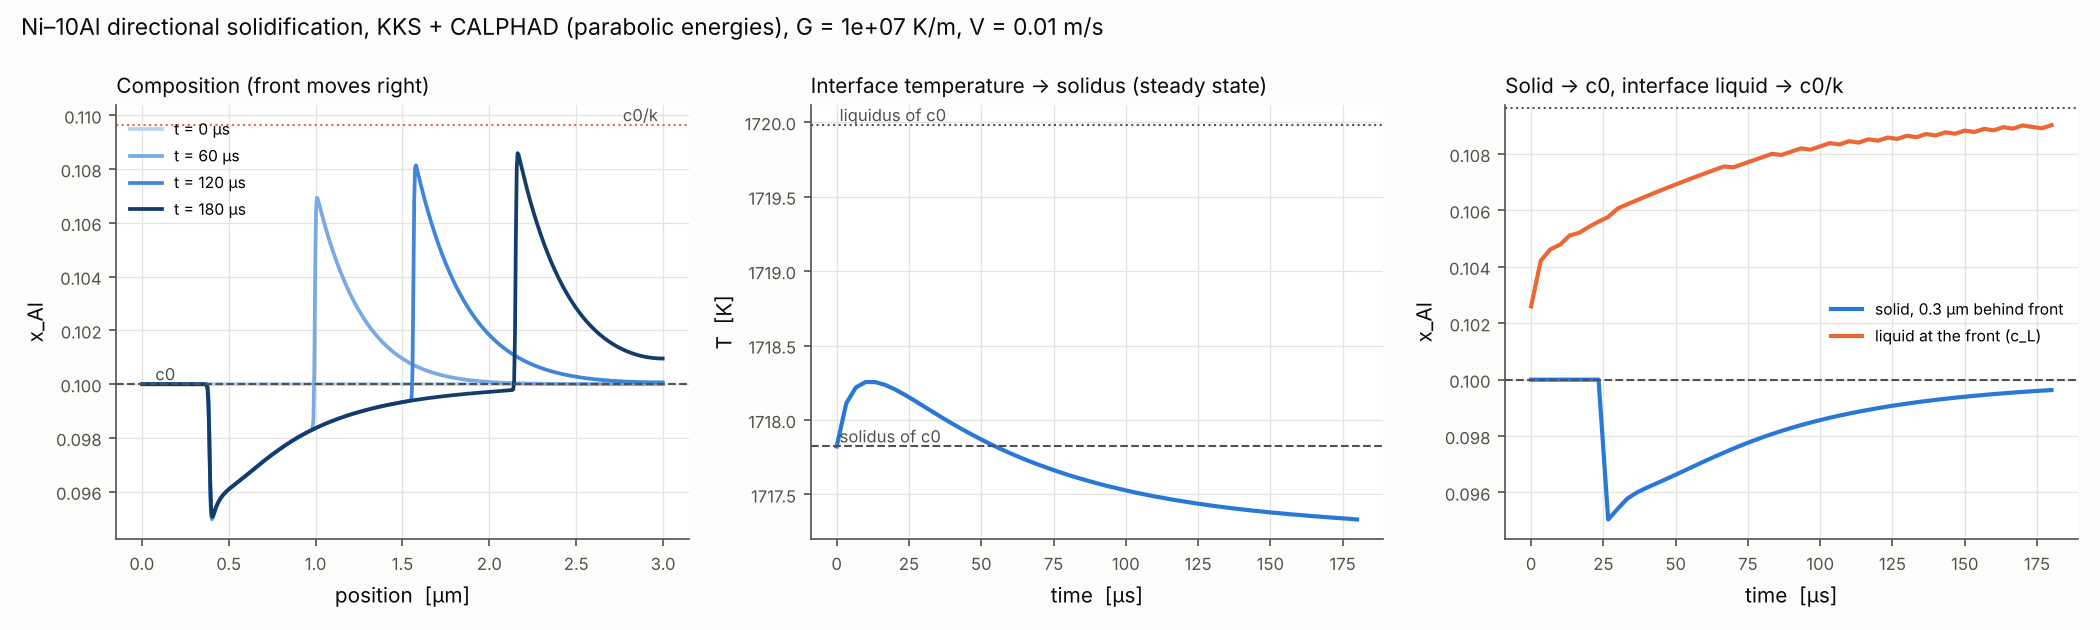
\includegraphics[width=\textwidth]{kks_1d_parabolic.png}
\caption{Ni--10Al directional solidification with KKS and CALPHAD parabolic energies: composition profiles, interface temperature and interface compositions over time}
\label{fig:kks-demo}
\end{figure}
This is the textbook steady state of a flat front, and the same checks are worth running on any code you write:

\begin{itemize}
\item Solute is conserved to round-off (drift 7 \(\times\) 10\(^{-14}\)).
\item The solid forms at the alloy composition, c0 = 0.10 (0.0996, still approaching).
\item The liquid at the front approaches c0/k = 0.1096.
\item The front sits just below the solidus, by 0.5 K of kinetic undercooling, and moves at the imposed speed V.
\end{itemize}

\needspace{7\baselineskip}
\subsection*{8.10 From your own code}
\addcontentsline{toc}{subsection}{8.10 From your own code}
Inside a Python code, use \texttt{KKSModel} directly, as the demo does. From C++ there are two routes (reference \S{}9):

\begin{itemize}
\item \textbf{Parabolic, no server at run time.} In Python, once: \texttt{kks.\allowbreak{}export\_\allowbreak{}parabolic\_\allowbreak{}csv(\textquotedbl{}tie\_\allowbreak{}lines.\allowbreak{}csv\textquotedbl{},\allowbreak{} temps)}. \texttt{cpp/\allowbreak{}kks\_\allowbreak{}parabolic.\allowbreak{}hpp} reads that file and does the split and the driving force in C++.
\item \textbf{Over HTTP.} \texttt{POST /\allowbreak{}kks/\allowbreak{}parameters} once at start-up returns the tie lines and, if asked, tables of G, G\('\) and G\(''\).
\end{itemize}
Either way, fetch the thermodynamics once at start-up. Never call the server at every grid point and time step: one API call takes 0.1--1 s (Part 7), while the demo's entire time step takes 158 \(\mu\)s.


\needspace{7\baselineskip}
\subsection*{Key ideas}
\begin{itemize}
\item \(\phi\) marks the phases; the interface is where \(\phi\) is between 0 and 1.
\item KKS splits the composition at every point into \(c_{S}\) and \(c_{L}\) with equal diffusion potentials: Part 2's common tangent, applied locally.
\item \(\Delta\)F, the gap between the two parallel tangents, drives the interface. It is zero at equilibrium.
\item CALPHAD enters only as f, f\('\) and f\(''\) of each phase. \texttt{calphad\_\allowbreak{}kks.\allowbreak{}py} supplies them three ways: exact, table, parabolic.
\item Check every simulation: solute conserved, the right compositions far from and at the interface.
\end{itemize}

\needspace{7\baselineskip}
\subsection*{Exercises}
\textbf{8.1} Compute \(\varepsilon ^{2}\) and W for \(\sigma\) = 0.18 J/m\(^{2}\) and a width of 10 nm. Check both formulas of 8.2 with your numbers.

\textbf{8.2} Evaluate \texttt{KKSModel.\allowbreak{}h} and \texttt{KKSModel.\allowbreak{}dh} at \(\phi\) = 0, 0.5 and 1. Why must h\('\) be zero at both ends?

\textbf{8.3} In the 1500 K table, c changes across the interface but \(c_{S}\) and \(c_{L}\) do not. Why? What would the naive blend of 8.3 do instead?

\textbf{8.4} Convert the 1490 K driving force in the bulk solid, \(-\)1.41 \(\times\) 10\(^{7}\) J/m\(^{3}\), to J/mol with \(V_{m}\) = 7.1 \(\times\) 10\(^{-6}\) m\(^{3}\)/mol.

\textbf{8.5} Why does \texttt{mode=\textquotedbl{}parabolic\textquotedbl{}} need a list of temperatures while \texttt{mode=\textquotedbl{}exact\textquotedbl{}} does not?

\textbf{8.6} You want a KKS model of \(\gamma\) (\texttt{FCC\_\allowbreak{}A1}) and \(\gamma '\) (\texttt{FCC\_\allowbreak{}L12}) in Ni--Al. Which mode do you choose, and what happens if you try \texttt{\textquotedbl{}exact\textquotedbl{}}?


\needspace{10\baselineskip}
\section*{Part 9 --- Putting it together}
\addcontentsline{toc}{section}{Part 9 --- Putting it together}
This part runs one realistic job from start to finish: preparing the thermodynamics of a solidification simulation of Ni--10Al, the alloy of Part 8's demo. Every step is one API call, and every result is read with the habits of Parts 2, 6 and 7. Start the server as in 7.9, then run:

\begin{lstlisting}[basicstyle={\scriptsize\ttfamily},language=Python]
from calphad_client import CalphadClient

c = CalphadClient("http://127.0.0.1:8000", db="alni_dupin_2001")

# Step 1: where does Ni-10Al solidify?
r = c.equilibrium({"AL": 0.10}, T=[1700, 1716, 1718, 1719, 1720, 1722], balance="NI")
for res in r["results"]:
    print(res["T"], [(p["phase"], p["state"], p["equivalent_to"], round(p["fraction"], 3),
                      round(p["composition"]["AL"], 4)) for p in res["phases"]],
          "verified:", res["stability_check"]["verified"])

# Step 2: which phases are close to forming at 1718 K?
r2 = c.phase_energies({"AL": 0.10}, T=1718, balance="NI")
print("\nstable:", r2["stable_phases"])
for p in r2["phases"]:
    if p["GM"] is not None:
        print(f"{p['phase']:8s} above eq {p['GM_above_equilibrium']:8.2f}  driving force {p['driving_force']:9.2f}  state {p['state']}")

# Step 3: KKS inputs for FCC_A1 + LIQUID
k = c.kks_parameters(solute="AL", phase_a="FCC_A1", phase_b="LIQUID",
                     T=[1705, 1710, 1715, 1718], mode="parabolic", c_alloy=0.10, Vm=7.0e-6)
print("\nwarnings:", k["warnings"])
for row in k["tie_lines"]:
    print({key: round(row[key], 4) for key in ("T", "c_a", "c_b", "k", "mu", "A_a", "A_b")},
          "consistent:", row["consistent"])
\end{lstlisting}
\begin{lstlisting}[basicstyle={\scriptsize\ttfamily}]
1700.0 [('FCC_L12', 'disordered', 'FCC_A1', 1.0, 0.1)] verified: True
1716.0 [('FCC_L12', 'disordered', 'FCC_A1', 1.0, 0.1)] verified: True
1718.0 [('FCC_L12', 'disordered', 'FCC_A1', 0.934, 0.0994), ('LIQUID', None, None, 0.066, 0.1089)] verified: True
1719.0 [('FCC_L12', 'disordered', 'FCC_A1', 0.513, 0.0957), ('LIQUID', None, None, 0.487, 0.1046)] verified: True
1720.0 [('LIQUID', None, None, 1.0, 0.1)] verified: True
1722.0 [('LIQUID', None, None, 1.0, 0.1)] verified: True

stable: ['FCC_L12', 'LIQUID']
FCC_L12  above eq     0.06  driving force      0.00  state disordered
LIQUID   above eq    10.98  driving force      0.00  state None
BCC_B2   above eq  1433.04  driving force  -1420.51  state disordered

warnings: []
{'T': 1705.0, 'c_a': 0.134, 'c_b': 0.15, 'k': 0.8934, 'mu': -123310.1776, 'A_a': 332850.0346, 'A_b': 279860.0818} consistent: True
{'T': 1710.0, 'c_a': 0.1227, 'c_b': 0.1365, 'k': 0.8988, 'mu': -126973.7189, 'A_a': 329260.9461, 'A_b': 276972.4406} consistent: True
{'T': 1715.0, 'c_a': 0.1092, 'c_b': 0.1205, 'k': 0.9062, 'mu': -131340.2856, 'A_a': 326705.3524, 'A_b': 275599.5768} consistent: True
{'T': 1718.0, 'c_a': 0.0994, 'c_b': 0.1089, 'k': 0.9125, 'mu': -134505.9758, 'A_a': 326658.9513, 'A_b': 276698.5187} consistent: True
\end{lstlisting}
Reading it, step by step:

\begin{enumerate}
\item \textbf{The freezing range.} Ni--10Al is fully liquid at 1720 K and fully solid at 1716 K, so it freezes over about 2 K (the demo's solidus and liquidus, 1717.82 and 1719.98 K, fall inside these brackets). Every result is \texttt{verified}. The solid is reported as \texttt{FCC\_\allowbreak{}L12}, but \texttt{state} is \texttt{disordered} and \texttt{equivalent\_\allowbreak{}to} is \texttt{FCC\_\allowbreak{}A1}: it is \(\gamma\), not \(\gamma '\) (Part 6). That decides the phase name for the KKS model.
\item \textbf{The competition.} At 1718 K both \(\gamma\) and liquid sit on the tangent plane (driving force 0). B2 is 1420 J/mol short of forming, so a two-phase model is justified here. Their small \texttt{GM\_\allowbreak{}above\_\allowbreak{}equilibrium} values show the alloy composition is close to both phases' own compositions, as it should be inside a 2 K freezing range.
\item \textbf{The KKS inputs.} \texttt{FCC\_\allowbreak{}A1} + \texttt{LIQUID} (both one mixing sublattice, so exact and parabolic modes work), no warnings, every tie line consistent with pycalphad. k < 1: Al prefers the liquid, so the liquid ahead of a growing solid is enriched in Al. The 1718 K tie line matches step 1's phase compositions, 0.0994 and 0.1089. Here \texttt{mu} is \(\mu_{\mathrm{Al}}\) \(-\) \(\mu_{\mathrm{Ni}}\).
\end{enumerate}
What would come next: interface parameters from \(\sigma\) and the grid (8.2), a 1-D run with the checks of 8.9, and only then 2-D or 3-D.


\needspace{7\baselineskip}
\subsection*{9.1 A workflow for any new alloy}
\addcontentsline{toc}{subsection}{9.1 A workflow for any new alloy}
\begingroup\small
\begin{longtable}{>{\raggedright\arraybackslash}p{0.245\linewidth}>{\raggedright\arraybackslash}p{0.268\linewidth}>{\raggedright\arraybackslash}p{0.408\linewidth}}
\toprule
\textbf{Step} & \textbf{Call} & \textbf{Look at} \\
\midrule
\endhead
1. Meet the database & \texttt{GET /\allowbreak{}databases/\allowbreak{}\{name\}} or \texttt{info()} & Phases, sublattices, order/disorder pairs (Part 4, 7.3) \\
2. Find the freezing range & API 1 with a list of T & Phases, fractions, \texttt{state}, \texttt{equivalent\_\allowbreak{}to}, \texttt{verified} \\
3. Check the competition & API 2 at the temperatures you care about & Driving forces of absent phases \\
4. Look at the G curves (optional) & API 3 at one T & Which curves come close; \texttt{approximate} \\
5. Choose the KKS phases and mode & \texttt{KKSModel} or \texttt{/\allowbreak{}kks/\allowbreak{}parameters} & \texttt{warnings}, \texttt{consistent}, \texttt{T\_\allowbreak{}valid} \\
6. Test & A 1-D run & Conservation, compositions, interface temperature \\
\bottomrule
\end{longtable}
\endgroup

\needspace{7\baselineskip}
\subsection*{9.2 Before trusting a result}
\addcontentsline{toc}{subsection}{9.2 Before trusting a result}
\begin{itemize}
\item APIs 1 and 2: \texttt{stability\_\allowbreak{}check.\allowbreak{}verified} and \texttt{converged} are \texttt{true}.
\item Phase names: read \texttt{state} and \texttt{equivalent\_\allowbreak{}to}. A name listed twice has \texttt{composition\_\allowbreak{}set} 1 and 2.
\item API 2: \texttt{GM} of \texttt{null} means the phase cannot reach this composition. \texttt{splits\_\allowbreak{}if\_\allowbreak{}allowed} means it would rather separate into two.
\item API 3: \texttt{approximate: true} means sampled. Use API 2 at the compositions that matter, or raise \texttt{pdens}.
\item KKS: \texttt{warnings} is empty, every tie line is \texttt{consistent}, and your temperatures stay inside \texttt{T\_\allowbreak{}valid} for table and parabolic modes.
\end{itemize}

\needspace{7\baselineskip}
\subsection*{9.3 Where to look in the reference guide}
\addcontentsline{toc}{subsection}{9.3 Where to look in the reference guide}
The companion reference is the place to look up exact field names, options and limits.

\begingroup\small
\begin{longtable}{>{\raggedright\arraybackslash}p{0.522\linewidth}>{\raggedright\arraybackslash}p{0.264\linewidth}>{\raggedright\arraybackslash}p{0.134\linewidth}}
\toprule
\textbf{I want to \ldots{}} & \textbf{Use} & \textbf{Reference} \\
\midrule
\endhead
Install and start the server & \texttt{calphad\_\allowbreak{}server.\allowbreak{}py} & \S{}2 \\
Know the units and sign conventions &  & \S{}3 \\
Load another database, or list its phases & \texttt{POST /\allowbreak{}databases}, \texttt{GET /\allowbreak{}databases/\allowbreak{}\{name\}} & \S{}4 \\
Get stable phases, amounts and compositions; solidus and liquidus & API 1, \texttt{/\allowbreak{}equilibrium} & \S{}5 \\
Get the G of any phase, stable or not, and how close it is to forming & API 2, \texttt{/\allowbreak{}phase\_\allowbreak{}energies} & \S{}6 \\
Plot G curves or feed G(x) to my own model & API 3, \texttt{/\allowbreak{}energy\_\allowbreak{}surface} & \S{}7 \\
Set up a KKS model in Python & \texttt{KKSModel} & \S{}8 \\
Use KKS from C++ or over HTTP & \texttt{/\allowbreak{}kks/\allowbreak{}parameters}, \texttt{kks\_\allowbreak{}parabolic.\allowbreak{}hpp} & \S{}9 \\
Call the server from C++, MATLAB, Julia \ldots{} & HTTP + JSON & \S{}10 \\
Check the installation works & \texttt{selftest.\allowbreak{}py}, the 1-D demo & \S{}11 \\
Understand an error or a strange result &  & \S{}12 \\
\bottomrule
\end{longtable}
\endgroup

\needspace{7\baselineskip}
\subsection*{Exercises}
\textbf{9.1} Repeat step 1 for Ni--15Al, scanning 1680--1710 K in 2 K steps. Between which temperatures does it freeze, and as which phase?

\textbf{9.2} In step 1, the solid is called \texttt{FCC\_\allowbreak{}L12}. Which name do you give \texttt{KKSModel} for it, and why not \texttt{FCC\_\allowbreak{}L12}?

\textbf{9.3} Using k from the tie-line table (about 0.91), estimate the Al content of the first solid to form when Ni--10Al starts to freeze. Why is it below 0.10?


\needspace{10\baselineskip}
\section*{Glossary}
\addcontentsline{toc}{section}{Glossary}
Every term used in the code, the results and the reference guide, in plain words. The number in brackets is the part that explains it.

\begingroup\small
\begin{longtable}{>{\raggedright\arraybackslash}p{0.202\linewidth}>{\raggedright\arraybackslash}p{0.745\linewidth}}
\toprule
\textbf{Term} & \textbf{Meaning} \\
\midrule
\endhead
API & A set of operations a program offers to other programs. Here: equilibrium, phase energies, energy surfaces, and the KKS parameters (7). \\
\texttt{approximate} & API 3 flag: the G values were sampled, not minimised exactly, because the phase has several mixing sublattices (7.8). \\
Atomic percent & 100 \(\times\) mole fraction (2). \\
\texttt{balance} & The element that makes up whatever the others leave, e.g. \texttt{balance=\textquotedbl{}NI\textquotedbl{}} (7.4). \\
\texttt{calc\_\allowbreak{}opts}, \texttt{pdens} & Options for pycalphad's sampling. \texttt{pdens} is how many configurations it tries per phase (5, 6). \\
\texttt{calculate} & pycalphad function: G of a phase at configurations you choose or it samples. No minimisation (5). \\
CALPHAD & CALculation of PHAse Diagrams: write G of every phase as a fitted formula, then find the lowest-G state (3). \\
Chemical potential \(\mu _{i}\) & How much G changes when a little of element i is added. Equal in all coexisting phases. J/mol (2). \\
Common tangent & The line touching two G curves; its touching points are the tie-line ends (2). \\
Component & An element taking part in a calculation, plus \texttt{VA} if the database has vacancies (5). \\
Composition set & One copy of a phase in a result. A phase can appear twice, e.g. in a miscibility gap (6). \\
Conditions & The fixed quantities of a calculation: \texttt{v.\allowbreak{}T}, \texttt{v.\allowbreak{}P}, \texttt{v.\allowbreak{}N} and n \(-\) 1 of the \texttt{v.\allowbreak{}X} (5). \\
Constituent & A species allowed on a sublattice, listed in a \texttt{CONSTITUENT} line (4). \\
\texttt{consistent} & KKS tie-line flag: the polished tie line agrees with pycalphad's own (8.6). \\
\texttt{converged} & API 1 flag: the solver returned a complete answer (7.6). \\
Diffuse interface & An interface of finite width over which \(\phi\) changes smoothly (8.1). \\
Diffusion potential \(\tilde{\mu}\) & dG/dc = \(\mu_{\mathrm{solute}}\) \(-\) \(\mu_{\mathrm{solvent}}\) in a binary. Equal in both phases in KKS. The \texttt{mu} of the KKS module (8.3). \\
Disordered & All sublattices have the same composition, so the phase behaves like a simple solid solution (3). \\
\texttt{DormantPhase} & pycalphad tool: a phase's driving force against an existing equilibrium (7.5). \\
Double well W g(\(\phi\)) & Energy penalty for \(\phi\) between 0 and 1; gives the interface its energy (8.2). \\
Driving force & How far a phase's G curve dips below (positive) or stays above (negative) the equilibrium tangent plane, at its best composition. J/mol (6, 7.7). \\
\(\Delta\)F & KKS driving force: \(f_{S}\)(\(c_{S}\)) \(-\) \(f_{L}\)(\(c_{L}\)) \(-\) \(\tilde{\mu}\)(\(c_{S}\) \(-\) \(c_{L}\)). Negative: the solid grows (8.4). \\
Endpoint & An address on the server, such as \texttt{/\allowbreak{}equilibrium} (7.9). \\
Equilibrium & The state of lowest G at fixed T, P and overall composition (1, 2). \\
\texttt{equivalent\_\allowbreak{}to} & The phase name that describes the state found, e.g. \texttt{FCC\_\allowbreak{}A1} for disordered \texttt{FCC\_\allowbreak{}L12} (6). \\
Excess energy & The part of G beyond ideal mixing: how much unlike atoms attract or repel (3). \\
FastAPI & The Python library the server is built with (7.9). \\
\texttt{FUNCTION} & A named, reusable expression in a TDB, e.g. \texttt{GHSERNI} (4). \\
G, \texttt{GM} & Gibbs energy; \texttt{GM} is per mole of atoms. J/mol (1). \\
\texttt{GM\_\allowbreak{}above\_\allowbreak{}equilibrium} & API 2: G of the phase alone at the alloy composition minus G of the equilibrium. Never negative (7.7). \\
GHSER & The SGTE reference energy of a pure element, the zero from which G is measured (4). \\
Gradient energy \(\varepsilon ^{2}\) & Coefficient of the gradient term (\(\varepsilon ^{2}\)/2)|\(\nabla \phi\)|\(^{2}\); with W it sets the interface width and energy (8.2). \\
h(\(\phi\)) & Interpolation function \(\phi ^{3}\)(6\(\phi ^{2}\) \(-\) 15\(\phi\) + 10), flat at both ends (8.1). \\
HTTP status code & The number a server returns: 200 success, 400 bad input, 404 unknown database, 422 malformed request, 500 internal error (7.9). \\
Ideal mixing & RT[x ln x + (1 \(-\) x) ln(1 \(-\) x)]: the entropy gain of mixing atoms at random (1). \\
Interface energy \(\sigma\) & Energy per area of a solid--liquid interface. J/m\(^{2}\) (8.2). \\
\texttt{IsolatedPhase} & pycalphad tool: one phase minimised on its own as a single homogeneous phase (7.5). \\
JSON & The text format of requests and responses: \texttt{\{\}} dictionaries, \texttt{[]} lists (7.9). \\
KKS & Kim--Kim--Suzuki: a phase-field model that splits c into \(c_{S}\) and \(c_{L}\) at equal diffusion potential (8). \\
Lever rule & Phase fractions from the tie line: \(f_{L}\) = (\(c_{S}\) \(-\) c)/(\(c_{S}\) \(-\) \(c_{L}\)) (2). \\
Liquidus, solidus & Temperatures where an alloy starts and finishes freezing (2). \\
Miscibility gap & A single phase separating into two compositions (3). \\
\texttt{Model} & pycalphad object holding one phase's symbolic G formula, \texttt{GM} (5). \\
Molar volume \(V_{m}\) & m\(^{3}\)/mol. Converts J/mol to J/m\(^{3}\) (8.2). \\
Mobility M & How quickly \(\phi\) responds to its driving force (8.4). \\
Mole fraction x & Fraction of atoms of an element (1). \\
\texttt{NP} & Phase fraction in a pycalphad result (5). \\
Order parameter \(\phi\) & Phase-field variable: 1 in phase a (solid), 0 in phase b (liquid) (8.1). \\
Ordered & Sublattices have different compositions, e.g. \(\gamma '\) (L1\(_{2}\)) or B2 (3). \\
Order/disorder pair & An ordered phase and its disordered partner described by one set of parameters, e.g. \texttt{FCC\_\allowbreak{}L12} and \texttt{FCC\_\allowbreak{}A1} (3, 4). \\
Parabolic approximation & G \(\approx\) \(G_{\mathrm{eq}}\) + \(\mu_{\mathrm{eq}}\)(c \(-\) \(c_{\mathrm{eq}}\)) + (A/2)(c \(-\) \(c_{\mathrm{eq}}\))\(^{2}\) near the tie line (8.5). \\
Partition coefficient k & \(c_{S}\)/\(c_{L}\) on the tie line. Below 1: the solute is pushed into the liquid (8.6). \\
Phase & A region with one structure and smoothly varying composition: liquid, FCC, B2 \ldots{} (1). \\
pycalphad & The Python library that reads TDB files and computes equilibria (5). \\
Redlich--Kister L\(_{0}\), L\(_{1}\) \ldots{} & Coefficients of the excess energy, usually a + bT (3, 4). \\
Site fraction y & Fraction of a sublattice's sites held by one species (3). \\
Site ratio & Number of sites on each sublattice, e.g. 0.75 : 0.25 for L1\(_{2}\) (3, 4). \\
\texttt{splits\_\allowbreak{}if\_\allowbreak{}allowed} & API 2: the phase on its own would rather separate into two compositions (7.7). \\
\texttt{stability\_\allowbreak{}check} & API 1 and 2: driving forces of absent phases; \texttt{verified} when all are \(\le\) 1 J/mol (6, 7.6). \\
\texttt{state} & \texttt{ordered} or \texttt{disordered} for order/disorder phases, \texttt{null} otherwise (6). \\
Stoichiometric compound & A phase that exists at one composition only, e.g. \texttt{AL3NI1} (3). \\
Sublattice & A set of equivalent sites in a crystal, filled independently (3). \\
TDB & The text file format of a thermodynamic database (4). \\
Tie line & The horizontal line joining two coexisting phase compositions on a phase diagram (2). \\
\texttt{VA} & Vacancy: an empty site. Needed as a component when any phase has vacancy sublattices (4, 5). \\
\texttt{vertex} & pycalphad dimension holding the slots for coexisting phases; empty slots are \texttt{\textquotesingle{}\textquotesingle{}} (5). \\
\texttt{Workspace} & pycalphad object that solves an equilibrium once and answers property queries (7.5). \\
xarray Dataset & NumPy arrays sharing named dimensions; what \texttt{equilibrium} returns (5). \\
\bottomrule
\end{longtable}
\endgroup

\needspace{10\baselineskip}
\section*{Answers to the exercises}
\addcontentsline{toc}{section}{Answers to the exercises}

\needspace{7\baselineskip}
\subsection*{Part 1}
\textbf{1.1} At 1300 K the solid is lower by 562.6 J/mol. At 1400 K the liquid is stable, by 413.4 J/mol.

\textbf{1.2} \(-\)7013.3 J/mol at x = 0.25, more negative than \(-\)4054.3 J/mol at x = 0.1. Mixing entropy is largest at x = 0.5.

\textbf{1.3} The slope of x ln x is ln x + 1, which goes to \(- \infty\) as x \(\rightarrow\) 0. Any finite energy cost of the first solute atoms is beaten by this infinitely steep drop, which is why no real metal is perfectly pure.

\textbf{1.4} The liquid has the higher G, so the solid is stable. The size of the value is how much the solid is favoured.


\needspace{7\baselineskip}
\subsection*{Part 2}
\textbf{2.1} At 1550 K the liquid has \(x_{\mathrm{Ni}}\) = 0.395 and the FCC 0.542. \(f_{L}\) = (0.542 \(-\) 0.5)/(0.542 \(-\) 0.395) = 0.286. API 1 gives 0.2858.

\textbf{2.2} One phase: liquid. At 1500 K, \(x_{\mathrm{Ni}}\) = 0.20 lies left of the liquid end of the tie line (0.270).

\textbf{2.3} From where \(\mu_{\mathrm{Ni}}\) is higher (the liquid) to where it is lower (the FCC). They stop when \(\mu_{\mathrm{Ni}}\) is equal in both, which is equilibrium.

\textbf{2.4} About 60 J/mol: the liquid alone at \(x_{\mathrm{Ni}}\) = 0.33 is \(-\)86 975.2 J/mol, the liquid + FCC mixture \(-\)87 035.4 J/mol.


\needspace{7\baselineskip}
\subsection*{Part 3}
\textbf{3.1} A positive L means Cu and Ni prefer like neighbours. At low temperature, where \(-\)TS is weak, the FCC splits into two. At 500 K, Cu--50Ni gives FCC with \(x_{\mathrm{Ni}}\) = 0.217 (61.3\%) and FCC with \(x_{\mathrm{Ni}}\) = 0.948 (38.7\%). At 600 K the two are 0.393 and 0.807. By 700 K the gap has closed.

\textbf{3.2} 3499.3 J/mol. L\(_{1}\) is multiplied by (\(x_{\mathrm{Cu}}\) \(-\) \(x_{\mathrm{Ni}}\)), which is zero at x = 0.5.

\textbf{3.3} \(x_{\mathrm{Al}}\) = 0.75 \(\times\) 0.10 + 0.25 \(\times\) 0.70 = 0.25. The two sublattices differ, so it is ordered.

\textbf{3.4} \texttt{AL3NI1} is a stoichiometric compound fixed at \(x_{\mathrm{Al}}\) = 0.75. It cannot exist at 0.25.


\needspace{7\baselineskip}
\subsection*{Part 4}
\textbf{4.1} \texttt{PHASE LIQUID \% 1 1.\allowbreak{}0} with \texttt{CONSTITUENT LIQUID :AL,\allowbreak{}NI :}: one sublattice holding Al or Ni. \texttt{PHASE BCC\_\allowbreak{}B2 \%( 3 .\allowbreak{}5 .\allowbreak{}5 3} with \texttt{CONSTITUENT BCC\_\allowbreak{}B2 :AL,\allowbreak{}NI,\allowbreak{}VA : AL,\allowbreak{}NI,\allowbreak{}VA : VA :}: three sublattices in ratio 0.5 : 0.5 : 3. The first two hold Al, Ni or vacancies; the third only vacancies (the interstitial sites).

\textbf{4.2} The first-order Redlich--Kister interaction between Cu and Ni in FCC, with vacancies on the second sublattice. At 1500 K it is \(-\)545.59 J/mol.

\textbf{4.3} They are equal, to within rounding: 1357.77 K is the melting point of Cu. The TDB switches expression there because the description of each phase changes form at the melting point.

\textbf{4.4} \texttt{G(FCC\_\allowbreak{}L12,\allowbreak{}NI:AL:VA;0)}: Ni on the 3/4 sublattice, Al on the 1/4 sublattice, which is perfectly ordered Ni\(_{3}\)Al.


\needspace{7\baselineskip}
\subsection*{Part 5}
\textbf{5.1} \texttt{FCC\_\allowbreak{}A1} needs \texttt{VA} on its second sublattice, so without it pycalphad silently drops the phase. The result is 100\% liquid: wrong, and with no error message. The framework adds \texttt{VA} for you.

\textbf{5.2} Two phases from 1540 to 1580 K (liquid fraction 0.098 at 1540 K, 0.881 at 1580 K), all FCC at 1530 K and all liquid at 1590 K. Melting starts between 1530 and 1540 K and ends between 1580 and 1590 K.

\textbf{5.3} \texttt{points=[[0.\allowbreak{}67,\allowbreak{} 0.\allowbreak{}33,\allowbreak{} 1.\allowbreak{}0]]}: Y(Cu), Y(Ni) on the first sublattice, then Y(VA) on the second. G = \(-\)86 970.39 J/mol, the same as API 2's FCC value.

\textbf{5.4} At equilibrium each element has the same chemical potential in every phase present (Part 2). So there is one \(\mu\) per element for the whole system, while each phase has its own composition.


\needspace{7\baselineskip}
\subsection*{Part 6}
\textbf{6.1} \texttt{verify=False}: L1\(_{2}\) + liquid, GM = \(-\)118 162.44 J/mol, check not run. \texttt{verify=True}: L1\(_{2}\) + B2, GM = \(-\)118 173.48 J/mol, verified at 2000 samples. The second is right: it is 11.04 J/mol lower, and its check shows every absent phase below the tangent plane.

\textbf{6.2} The first has Al site fractions 0.0006 and 0.9469 on its two sublattices: Ni on one, Al on the other, ordered \(\gamma '\). The second has 0.1246 on both: disordered \(\gamma\).

\textbf{6.3} The liquid's G curve stays 26.09 J/mol above the tangent plane even at its best composition, so it cannot form. +5.0 would mean some liquid composition lies 5 J/mol below the plane: the result is not the minimum, and the framework would re-solve.

\textbf{6.4} Equilibrium is the minimum of G. A calculation can miss a lower state but cannot produce a state below the true minimum, so of two valid answers the lower one is closer to the truth.


\needspace{7\baselineskip}
\subsection*{Part 7}
\textbf{7.1} \(x_{\mathrm{Ni}}\) = 0.3170, \(x_{\mathrm{Cu}}\) = 0.6830. By hand: 30/58.69 = 0.5112 mol Ni, 70/63.546 = 1.1016 mol Cu, \(x_{\mathrm{Ni}}\) = 0.5112/1.6128 = 0.3170.

\textbf{7.2} Ni, the largest. Mole fractions sum to 1, so \(x_{\mathrm{Ni}}\) = 1 \(-\) 0.2 \(-\) 0.1 is fixed by the other two.

\textbf{7.3} \texttt{GM\_\allowbreak{}above\_\allowbreak{}equilibrium} compares B2 at the alloy's own composition, \(x_{\mathrm{Al}}\) = 0.25. The driving force compares B2 at its best composition, richer in Al, with the tangent plane. The driving force tells you how close B2 is to forming: 98 J/mol, not 292.

\textbf{7.4} The liquid (0.270) + FCC (0.398) mixture lies on the common tangent; at \(x_{\mathrm{Ni}}\) = 0.33 both curves lie above that line. Each phase alone at the alloy composition is therefore 60--65 J/mol above the equilibrium, yet each touches the tangent at its own tie-line composition (driving force 0).

\textbf{7.5} 422, from FastAPI checking the body against \texttt{EquilibriumRequest}, where \texttt{T} is \texttt{Field(.\allowbreak{}.\allowbreak{}.\allowbreak{})}, required. The message names \texttt{[\textquotedbl{}body\textquotedbl{},\allowbreak{} \textquotedbl{}T\textquotedbl{}]}. No \texttt{CalphadSystem} code ran.

\textbf{7.6} \texttt{LIQUID} has one sublattice, so the composition fixes the site fractions and there is one exact G per composition. \texttt{FCC\_\allowbreak{}L12} has two mixing sublattices, so many arrangements share one composition; the grid keeps the lowest one sampled.


\needspace{7\baselineskip}
\subsection*{Part 8}
\textbf{8.1} \(\varepsilon ^{2}\) = 2.45 \(\times\) 10\(^{-9}\) J/m and W = 2.38 \(\times\) 10\(^{8}\) J/m\(^{3}\). Then \(\varepsilon \surd\)W/(3\(\surd\)2) = 0.180 J/m\(^{2}\) and 2.2\(\surd\)2 \(\varepsilon\)/\(\surd\)W = 10.0 nm.

\textbf{8.2} h = 0, 0.5, 1 and h\('\) = 0, 1.875, 0. If h\('\) were not zero at the ends, the bulk solid and liquid would feel \(\Delta\)F and \(\phi\) would drift away from 1 and 0 everywhere, not just at the interface.

\textbf{8.3} At equilibrium each phase sits at its own tie-line end; only the mixing fraction h changes across the interface, and c changes with it. The naive blend would force both phases to c, 62.83 J/mol above the equilibrium in the middle.

\textbf{8.4} \(-\)1.41 \(\times\) 10\(^{7}\) \(\times\) 7.1 \(\times\) 10\(^{-6}\) = \(-\)100 J/mol.

\textbf{8.5} Parabolic coefficients come from tie lines computed at the listed temperatures and interpolated between them. The exact mode evaluates the CALPHAD formula itself, which is valid at any T.

\textbf{8.6} \texttt{mode=\textquotedbl{}table\textquotedbl{}}, with \texttt{branches=\{\textquotedbl{}FCC\_\allowbreak{}L12\textquotedbl{}: \textquotedbl{}ordered\textquotedbl{}\}} for \(\gamma '\). \texttt{\textquotedbl{}exact\textquotedbl{}} raises: \texttt{FCC\_\allowbreak{}L12 has sublattices or vacancies mixing with the elements,\allowbreak{} so G at fixed composition needs an internal minimisation.\allowbreak{} Use mode=\textquotesingle{}table\textquotesingle{}.\allowbreak{}}


\needspace{7\baselineskip}
\subsection*{Part 9}
\textbf{9.1} Two phases from 1698 to 1704 K; all solid at 1696 K and all liquid at 1706 K. It freezes between about 1697 and 1705 K, a range four times wider than Ni--10Al's, as disordered \(\gamma\) (\texttt{FCC\_\allowbreak{}L12}, \texttt{state} disordered, \texttt{equivalent\_\allowbreak{}to} \texttt{FCC\_\allowbreak{}A1}).

\textbf{9.2} \texttt{FCC\_\allowbreak{}A1}. The state found is disordered \(\gamma\), and \texttt{FCC\_\allowbreak{}A1} has one mixing sublattice, so the exact and parabolic modes work. \texttt{FCC\_\allowbreak{}L12} has two, so \texttt{\textquotedbl{}exact\textquotedbl{}} refuses it.

\textbf{9.3} About k \(\times\) c\(_{0}\) = 0.91 \(\times\) 0.10 \(\approx\) 0.091 (the exact tie line at the liquidus gives 0.0918). It is below 0.10 because k < 1: Al prefers the liquid, so the first solid is Al-poor.


\needspace{10\baselineskip}
\section*{Further reading}
\addcontentsline{toc}{section}{Further reading}
In the order to read them, from foundations to the papers behind the code.

\textbf{Thermodynamics and phase diagrams}

\begin{itemize}
\item D. A. Porter, K. E. Easterling and M. Y. Sherif, \textit{Phase Transformations in Metals and Alloys}, CRC Press. Chapter 1 covers Parts 1--2 of this guide: G curves, common tangents, chemical potentials, ordering.
\end{itemize}
\textbf{CALPHAD}

\begin{itemize}
\item H. L. Lukas, S. G. Fries and B. Sundman, \textit{Computational Thermodynamics: The Calphad Method}, Cambridge University Press, 2007. \href{https://doi.org/10.1017/CBO9780511804137}{doi:10.1017/CBO9780511804137}. The standard text on the models of Part 3 and the TDB format of Part 4.
\item N. Dupin, I. Ansara and B. Sundman, ``Thermodynamic re-assessment of the ternary system Al--Cr--Ni'', \textit{Calphad} 25 (2001) 279--298. \href{https://doi.org/10.1016/S0364-5916(01)00049-9}{doi:10.1016/S0364-5916(01)00049-9}. The assessment behind the Ni--Al database used throughout.
\end{itemize}
\textbf{pycalphad}

\begin{itemize}
\item R. Otis and Z.-K. Liu, ``pycalphad: CALPHAD-based Computational Thermodynamics in Python'', \textit{Journal of Open Research Software} 5 (2017). \href{https://doi.org/10.5334/jors.140}{doi:10.5334/jors.140}.
\item The pycalphad documentation and examples: \href{https://pycalphad.org}{pycalphad.org}. Source code: \href{https://github.com/pycalphad/pycalphad}{github.com/pycalphad/pycalphad}.
\end{itemize}
\textbf{Phase-field and KKS}

\begin{itemize}
\item N. Moelans, B. Blanpain and P. Wollants, ``An introduction to phase-field modeling of microstructure evolution'', \textit{Calphad} 32 (2008) 268--294. \href{https://doi.org/10.1016/j.calphad.2007.11.003}{doi:10.1016/j.calphad.2007.11.003}. The best first read after Part 8, written for CALPHAD users.
\item W. J. Boettinger, J. A. Warren, C. Beckermann and A. Karma, ``Phase-field simulation of solidification'', \textit{Annual Review of Materials Research} 32 (2002) 163--194. \href{https://doi.org/10.1146/annurev.matsci.32.101901.155803}{doi:10.1146/annurev.matsci.32.101901.155803}.
\item S. G. Kim, W. T. Kim and T. Suzuki, ``Phase-field model for binary alloys'', \textit{Physical Review E} 60 (1999) 7186. \href{https://doi.org/10.1103/PhysRevE.60.7186}{doi:10.1103/PhysRevE.60.7186}. The KKS paper; Part 8 is a guided version of it.
\end{itemize}
\textbf{The tools around the code}

\begin{itemize}
\item FastAPI tutorial, for the server: \href{https://fastapi.tiangolo.com/tutorial/}{fastapi.tiangolo.com/tutorial}.
\item The companion reference guide, for every field, option and limit of this framework.
\end{itemize}

\end{document}
